%%%%%%%%%%%%%%%%%%%%%
%   AMS packages    %
%%%%%%%%%%%%%%%%%%%%%
\documentclass{amsart}

\usepackage{amsmath}
\usepackage{amsxtra}
\usepackage{amscd}
\usepackage{amsthm}
\usepackage{amsfonts}
\usepackage{amssymb}
\usepackage{eucal}
\usepackage[all]{xy}
\usepackage{graphicx}
\usepackage{tikz-cd}
\usepackage{mathrsfs}
\usepackage{subfiles}
\usepackage{mathpazo}
\usepackage{euler}
\usepackage{hyperref}
\usepackage{color}
\usepackage{longtable}
\usepackage{float}

\usepackage[colorinlistoftodos, textsize=tiny]{todonotes}
\def\listtodoname{List of Todos}
\def\listoftodos{\@starttoc{tdo}\listtodoname}

%\addtolength{\oddsidemargin}{-.5 in}
	%\addtolength{\evensidemargin}{-.4 in}
	%\addtolength{\textwidth}{1 in}
%
	%\addtolength{\topmargin}{0 in}
	%\addtolength{\textheight}{0 in}

\RequirePackage{color}
\definecolor{myred}{rgb}{0.75,0,0}
\definecolor{mygreen}{rgb}{0,0.5,0}
\definecolor{myblue}{rgb}{0,0,0.65}

%\usepackage{hyperref}
  %\hypersetup{colorlinks=true,citecolor=blue}

\usepackage{tikz}
\usepackage{tikz-cd}
\usetikzlibrary{matrix,arrows,decorations.pathmorphing}

%%%%%%%%%%%%%%%%%%%%%%% amsthm theorem styles %%%%%%%%
%%%%%%%%%%%%%%%

\theoremstyle{plain}
  \newtheorem{thm}{Theorem}[section]
  \newtheorem{prop}[thm]{Proposition}
  \newtheorem{lem}[thm]{Lemma}
  \newtheorem{cor}[thm]{Corollary}
	\newtheorem{claim}[thm]{Claim}
	\newtheorem{question}[thm]{Question}
	
\theoremstyle{definition}
  \newtheorem{defn}[thm]{Definition}
  \newtheorem{example}[thm]{Example}
  \newtheorem{exer}[thm]{Exercise}
  \newtheorem{ctexample}[thm]{Counterexample}
  \newtheorem{convention}[thm]{Convention}
	\newtheorem{conjecture}[thm]{Conjecture}
	
\theoremstyle{remark}
	\newtheorem{rem}[thm]{Remark}
  \newtheorem{note}[thm]{Notation}
  \newtheorem*{note*}{Notation}
  \newtheorem{case}{Case}
	
\numberwithin{equation}{section}

%%%%%%%%%%%%%%%%%%%%%%%%% custom commands %%%%%%%%%%%%%%%%%%%%%%%%%%%

\newcommand\nc{\newcommand}
\nc\on{\operatorname}
\nc\renc{\renewcommand}
\newcommand\ssec{\subsection}
\newcommand\sssec{\subsubsection}
\newcommand\bh{{\mathbb H}}
\newcommand\bO{{\mathbf O}}
\newcommand\CC{{\mathcal C}}
\newcommand\BN{{\mathbb N}}
\newcommand\BC{{\mathbb C}}
\newcommand\BF{{\mathbb F}}
\newcommand\BR{{\mathbb R}}
\newcommand\BQ{{\mathbb Q}}
\newcommand\BP{{\mathbb P}}
\newcommand\BBZ{{\mathbb Z}}
\newcommand\uR{\underline{R}}
\newcommand\uZ{\underline{\BBZ}}
\newcommand\CF{{\mathcal F}}
\newcommand\uCF{\underline{{\mathcal F}}}
\newcommand\BZ{{\mathbb Z}}
\newcommand\BA{{\mathbb A}}
\newcommand\fa{{\mathfrak a}}
\newcommand\fp{{\mathfrak p}}
\newcommand\fq{{\mathfrak q}}
\newcommand\fm{{\mathfrak m}}
\newcommand\so{{\mathscr O}}
\newcommand\sg{{\mathscr G}}
\newcommand \sx{\mathscr X}

\newcommand\scm{{\mathscr M}}
\newcommand\scn{{\mathscr N}}
\newcommand\scf{{\mathscr F}}
\newcommand\scg{{\mathscr G}}
\newcommand\sco{{\mathscr O}}
\newcommand\sch{{\mathscr H}}
\newcommand\scl{{\mathscr L}}
\newcommand\sci{{\mathscr I}}

\newcommand{\id}{\mathrm{id}}
\newcommand\im{\text{im }}
\newcommand\coker{\text{coker}}
\newcommand \spec{\text{Spec }}
\newcommand \proj{\text{Proj }}
\newcommand \rspec{\textit{Spec }}
\newcommand \rproj{\textit{Proj }}
\newcommand{\gal}{\mathrm{Gal}}

\newcommand \trdeg{\text{tr. deg }}
\newcommand \codim{\text{codim}}
\newcommand \rk{\text{rk }}
\newcommand \di{\text{div }}
\newcommand \depth{\text{depth }}
\DeclareMathOperator{\ord}{ord}
\DeclareMathOperator{\sym}{Sym}

%%%%%%%%%%%%%%%%%%%%% cring custom commands %%%%%%%%%%%%%%%%%%%%%%%%%

\newcommand \subhalf[1]{\frac{{#1} - 1}{2{#1}}}
\newcommand{\se}[1]{\section*{Problem #1}}
\newcommand \halfcan{L}
\newcommand \Supp{\text{Supp}}
\newcommand \initial{\text{in}}
\newcommand \gin{\text{gin}}
\newcommand \Eff{\text{Eff}}
\newcommand \sat{\text{sat}}

%%%%%%%%%%%%%%%%%%%%%%%%%%%%%% title %%%%%%%%%%%%%%%%%%%%%%%%%%%%%%%%

\title{Spin canonical divisors of log stacky curves}

\author{Aaron Landesman}
\address[Aaron Landesman]{Department of Mathematics, Harvard University}
\email{aaronlandesman@college.harvard.edu}

\author{Peter Ruhm}
\address[Peter Ruhm]{Department of Mathematics, Stanford University}
\email{pruhm@stanford.edu}

\author{Robin Zhang}
\address[Robin Zhang]{Department of Mathematics, Stanford University}
\email{robinz16@stanford.edu}

\date{\today}

%%%%%%%%%%%%%%%%%%%%%%%%%%%%%% document %%%%%%%%%%%%%%%%%%%%%%%%%%%%%%%%

\begin{document}

\begin{abstract}
  Arithmetic geometry group at the Emory University Number Theory
	REU.
\end{abstract}

\maketitle

\tableofcontents


%%%%%%%%%%%%%%%%%%%%%%%%%%%% Introduction %%%%%%%%%%%%%%%%%%%%%%%%%%%%%%%

\section{Introduction}
Let $\Gamma$ be a {\bf Fuchsian} subgroup, i.e. a discrete subgroup
of $PSL_2(\BR)$ acting on the upper half plane $\bh$ by fractional
linear transformations. We consider the {\bf ring of modular forms}
$M(\Gamma) = \bigoplus_k M_k(\Gamma)$. In this paper, for general
$\Gamma$, we sharply bound the degree of the generators and
relations for $M(\Gamma).$ The case where $M(\Gamma)$ has $M_{2k + 1
}(\Gamma) = 0$ for all $k \in \BZ$, i.e. when $\Gamma$ has no odd
weight modular forms, is answered in Voight and Zureick-Brown
\cite[Chapters 7-9]{vzb:stacky}. This work extends this result to
all Fuchsian subgroups $\Gamma$. In order to answer this question,
we translate the seemingly analytic question into the algebraic
category, using a generalization of the GAGA principle. By
\cite[Proposition 6.1.5]{vzb:stacky}, there is an equivalence of
categories between orbifold curves and log stacky curves over $\BC$
. Hence, for the remainder of the paper, we will work in the
algebraic category.

Let $X$ be a smooth algebraic curve over $k$ of genus $g$. It is
well known that the sheaf $\Omega _X,$ with associated divisor $K_X$
 determines the {\bf canonical map } $\pi:X \rightarrow \BP_k^{g - 1}$.
Then, the {\bf canonical ring} is defined to be
\begin{align*}
	R(X,K_X) = \bigoplus_{n \geq 0} H^0(X,nK_X),
\end{align*}

\noindent
with multiplication structure corresponding to tensor product of
sections. Since $\Omega_X$ is ample, $X \cong \proj R$. Petri's
theorem gives generators and relations for $R(X, K_X)$ showing that
in most cases $R(X, K_X)$ is generated in degree 1 with relations
in degree 2 (see \cite[p. 157]{saint-donat:proj}). This has the
pleasant geometric consequence that all such canonically embedded
curves are scheme theoretically cut out by quadratic equations

Following Voight and Zureick-Brown \cite{vzb:stacky}, we examine a
much more general setting, generalizing Petri's theorem in many
directions. A divisor $\Delta \in d X$ is a {\bf log divisor} if
$\Delta = \sum_{i}^{}P_i \in \di X,$ with all $P_i$ distinct. Let
$(\sx,\Delta)$ denote a tame separably rooted curve over a
field $k$ so that $X$ is the coarse space of $\sx$, as defined in
\cite[Section 5.2]{vzb:stacky} so that $\di \sx = \di X \bigoplus_{i
= 1}^r \langle \frac{1}{e_i}P_i \rangle,$ with $e_i \in \BZ$. Let $K_
\sx = K_X + \sum_{i = 1}^{r}\frac{e_i - 1}{e_i}P_i.$ In this case, we
say $\sx$ has {\bf stabilizer order} $e_i$ at $P_i$. Call $\halfcan
\in \di \sx$ a {\bf log half-canonical divisor} on $(\sx,\Delta)$,
be a divisor $\halfcan \in \di \sx$ so that $2\halfcan \sim K_\sx +
\Delta.$ If $X$ has genus $g$ and $\delta = \deg \Delta,$ then we
say $\sx$ has \textbf{signature} $(g; e_1, \ldots, e_r;\delta)$. A
{\bf log spin curve} is a triple $(X,\Delta,\halfcan)$ where $(X,\Delta)$
and $\halfcan$ is a log half-canonical divisor on $(\sx,\Delta)$.
The central object of study in this paper is the {\bf log spin
canonical ring} of $(X,\Delta,L)$ is
\begin{align*}
	R(X,\Delta,L) = \bigoplus_{n \geq 0} H^0(X,nL)
\end{align*}

\noindent
The main theorem of this paper is the following bound on the degree
of generators and relations of arbitrary log spin canonical rings:

\begin{thm}
\label{thm:general_generators_relations}
Let $(\sx, \Delta, \halfcan)$ log spin curve over a perfect field $k$, so
that $\sx$ has signature $\sigma = (0; e_1, \ldots, e_r; \delta)$. Then the
canonical ring

\begin{align*}
	R(\sx, \Delta, \halfcan) = \bigoplus_{d \geq 0} H^0(\sx, \sco(L)^{\otimes d})
\end{align*}

\noindent
is generated as a $k$-algebra by elements of degree at most $e =
\max(5, e_1, \ldots, e_r).$ If the genus $g \geq 2,$ and $\Delta = 0
$ then $R(\sx,\Delta, \halfcan)$ has relations generated in degrees
up to $\max(11, 2e_1, \ldots, 2e_r)$. Otherwise, $R(\sx, \Delta,
\halfcan)$ has relations generated in degrees up to $\max(10, 2e_1,
\ldots, 2e_r),$ so long as $\sigma$ does not lie in a finite list
of exceptional cases, as listed in Table ~\ref{table:g-1-exceptional}
for signatures with $g = 1$ and Table ~\ref{table:g-0-exceptional}
for signatures with $g = 0$.
\end{thm}

\todo{Say that this follows immediately from the three theorems for the special cases.}

Note that in the course of the proof of Theorem
~\ref{thm:g_0_generators_relations} we will not merely obtain
bounds on the degrees of the generators and relations. In fact, if
the genus $g = 0$ or $g = 1$, the proof yields an explicit system
of generators and the initial ideal of relations. While in the
genus $g \geq 2$ case, the proof does not always yield an explicit
system of generators and relations, if the halfcanonical divisor
$\halfcan$ can be written as $\halfcan' + \Lambda$ with $(\halfcan',
0, X)$ a log spin curve, and a system of generators and relations for
$ \halfcan'$ is known, then our proof provides an inductive
procedure for determining the generators and initial ideal of
relations for $\halfcan$. In fact, such a system of generators and
relations are known for $\halfcan'$ in many cases, as detailed in
Neves ~\cite[ Section III.4]{neves:halfcan}.

The remainder of the paper will be primarily devoted to proving
Theorem ~\ref{thm:general_generators_relations}. The idea of the
proof will be to induct on the order and number of elliptic points.
To this end, we first review important background in Section
~\ref{sec:background}. Then, in Section ~\ref{sec:induction}, we
develop various inductive tools. In Sections ~\ref{sec:g_high},
~\ref{sec:g_1} and ~\ref{sec:g_0}, we prove Theorem
~\ref{thm:general_generators_relations} in the cases that the genus
$g \geq 2, g = 1$ and $g = 0$ respectively. Finally, in Section
~\ref{sec:further-questions}, we pose several questions for future
research.

%%%%%%%%%%%%%%%%%%%%%%%%%%%% Background %%%%%%%%%%%%%%%%%%%%%%%%%%%%%%%

\section{Background}
\label{sec:background}
Look at Spencer-Kodaira \cite{kodaira:complex-manifolds}.
Include the following:
\begin{enumerate}
	\item Note that this result is independence of base field
	\item background on Gr\"{o}bner bases
	\item Notation $h^0 = \dim H^0$.
	\item Why we have these fractions $\frac{e_i - 1}{2e_i}$ and why $e_i$ must be odd.
\end{enumerate}

\subsection{Junk}
This is stuff that has been moved out of the introduction to possibly
be retooled for this section.

We can then consider the
orbifold $\Gamma \backslash \bh$ over $\BC$. For example, in the
case $\Gamma$ acts freely on $\bh$, $\Gamma \backslash \bh$ is a
Riemann Surface over $\BC$. It may well be that $\Gamma \backslash
\bh$ is not compact. Defining $\Delta$ as the divisor of cusps
associated to $\Gamma$, we can form a space $\Gamma \backslash
\bh^*$ which is a compactification of $\Gamma \backslash \bh,$ with
associated {\bf divisor of cusps} $\Delta$.

\subsection{Definitions}
We reserve the notation $\halfcan$ for the halfcanonical divisor
where $\halfcan \sim $.

Here are some definitions.

We define the notion of the saturation of a divisor, taken from
Voight and Zureick-Brown ~\cite[Section 7.2]{vzb:stacky}.

\begin{defn}
Let $D$ be a divisor on $\sx$. The \textbf{effective monoid} of $D$
is the monoid
\[
	\Eff(D) = \{d \in \BZ_{\geq 0} : \deg \lfloor dD \rfloor \geq 0 \}
\]
\end{defn}

\begin{defn}
\label{defn:sat}
The \textbf{saturation} for a monoid $M \subseteq \BZ_{\geq 0}$,
denoted $\sat(M)$, is the smallest integer $s$ such that $M
\supseteq \BZ_{\geq s}$, if such an integer exists.
\end{defn}

\begin{rem}
For our purposes, it is useful to call the saturation of the
effective monoid of a divisor $D$ as the saturation $s$ of the
divisor $D$ on $\sx$. In this case, the saturation $s$ of a divisor
$D$ on $\sx$ (i.e. $\sat(\Eff(D))$) is the smallest positive $s \in
\BZ$ such that $\deg \lfloor dD \rfloor \geq 0$ for all $d \geq s$.
\end{rem}



%%%%%%%%%%%%%%%%%%%%%%%%%%% Inductive Lemmata %%%%%%%%%%%%%%%%%%%%%%%%%%%%%%%


\section{Inductive Lemmata}
\label{sec:induction}
First we present the general inductive Lemmata that will be applied
for all genera. We offer various inductive Lemmata that will allow
us to add fractional point $\frac{\alpha}{\beta}P$ to a $\BQ$
 divisor $D$ of $X$ and describe the new generators and relations
of $R_{D + P}$ not in $R_D$. Next, we provide a method specific to
the case of stacky canonical divisors, which
under certain conditions allows us to transfer information about
the generators and relations of the half canonical ring of a stacky
curve $\sx$' with signature $(g; e_1', \ldots, e_\tau'; 0)$ to a
stacky curve $\sx$ with signature $(g; e_1, \ldots, e_\tau; 0)$
where each $e_i\in \{e_i', e_i' + 2\}$.   

However, before we can answer these general Lemmata, it is useful
to prove a nice result about minimal generation of ideals of
relations.

\todo{Include one of the following, if the first one, include a 
remark for quotient}

%\begin{lem}
%\label{lem:minimal_quadratic}
%Suppose $k[x_1, \ldots, x_n]$ is a graded ring, not necessarily
%generated in degree 1, is equipped with a monomial ordering $\prec$.
 %Let $\phi:k[x_1, \ldots, x_n] \rightarrow B'$ be a map of graded
%rings with kernel $I'$, such that $I'$ is generated by elements $f_1,
%\ldots, f_j$, where $in_\prec(f_i) = x_i x_j,$ and no term of $f_i$
%is of the form $x_k$. Then, the elements $f_i$ determine minimal
%generators for $I$.
%\end{lem}
%\begin{proof}
%Regrade the ring $k[x_1, \ldots, x_n]$ so that all $x_i$ lie in
%degree 1. Then,
%\[
	%\phi : k[x_1, \ldots, x_n] \rightarrow B
%\]
%\noindent
%determines a map of rings, no longer necessarily graded. Consider
%the grlex monomial ordering $\prec$ on $k[x_1, \ldots, x_n]$.
%\todo{This ordering isn't quite right. 
%We need to preserve the ordering on quadratic terms}
%By
%assumption, the kernel $I$ is generated by elements whose initial
%terms have degree 2 and are all distinct. Therefore, $\dim_k (k[x_1,
%\ldots, x_n])_2 = \binom{n}{2} - j.$ This implies any set of
%generators for $I$ must have at least $j$ elements. Since $f_1,
%\ldots, f_j$ is such a set, it is minimal.
%\end{proof}
%
%\begin{rem}
%In particular, in the case of
%\[
	%\begin{tikzcd}
		%I\ar[hookrightarrow]{r}\ar[hookrightarrow]{d} & k[x_1, \ldots, x_n]
		%\ar[twoheadrightarrow]{r} \ar[hookrightarrow]{d} & B \ar[hookrightarrow]{d} \\
		%I' \ar[hookrightarrow]{r} & k[x_1, \ldots, x_n, y_1, \ldots, y_m] \ar[twoheadrightarrow]{r}& B'
	%\end{tikzcd}
%\]
%inducing
%\[
	%I/I'\hookrightarrow k[y_1, \ldots, y_m]\twoheadrightarrow B'/B
%\]
%\todo{how do we make this proof?}
%\end{rem}

\begin{lem}
\label{lem:minimal_quadratic}
Suppose $k[x_1, \ldots, x_n]\hookrightarrow k[x_1, \ldots, x_n, y_1, \ldots, y_m]$ be graded ring, not necessarily
generated in degree 1 that are equipped with monomial ordering $\prec$.
Let $\phi: k[x_1, \ldots, x_n] \twoheadrightarrow B, \phi':k[x_1, \ldots, x_n, y_1, \ldots, y_m]\twoheadrightarrow B'$ be maps of graded
rings with kernels $I \hookrightarrow I'$ such that the following diagram commutes:
\[
	\begin{tikzcd}
	I\ar[hookrightarrow]{r}\ar[hookrightarrow]{d} & k[x_1, \ldots, x_n]\ar[twoheadrightarrow]{r} \ar[hookrightarrow]{d} & B \ar[hookrightarrow]{d}\\
	I' \ar[hookrightarrow]{r} & k[x_1, \ldots, x_n, y_1, \ldots, y_m] \ar[twoheadrightarrow]{r}& B'
	\end{tikzcd}
\]
Further suppose that $I'$ is generated over $I$ by elements $f_1,
\ldots, f_j$ as a $k$-vector space, where $in_\prec(f_i) \in \{y_i x_j, y_i y_j\}$ and no monomial of $f_i$
is of the form $y_i$. Then, the elements $f_i$ determine minimal
generators for $I'$ over $I$.
\end{lem}

\begin{proof}
Regrade the rings $k[x_1, \ldots, x_n], k[x_1, \ldots, x_n, y_1, \ldots, y_m]$ so that all $x_i$ and $y_j$ lie in
degree 1. Then,
\[
	\phi : k[x_1, \ldots, x_n] \twoheadrightarrow B 
\]
\[
	\phi': k[x_1, \ldots, x_n, y_1, \ldots, y_m] \twoheadrightarrow B'
\]


\noindent
determines map of rings, no longer necessarily graded. 
By assumption, $I'$ is generated over $I$ as a $k$-vector space by elements $f_1, \ldots, f_n$ whose initial terms have degree 2 and are linearly independent. By the theory of Gr\"{o}bner basis,
\[
	\dim_k(B'/B)_2=\dim_k(k[x_1, \ldots, x_n, y_1, \ldots, y_m]/k[x_1, \ldots, x_n])_2 - j
\]
so
\[
	\dim_k (I'/I)_2=j.
\]
This implies any set of
generators for $I$ must have at least $j$ elements. Since $f_1,
\ldots, f_j$ is such a set, it is minimal.
\end{proof}


\begin{rem}
\label{rem:minimal_quadratic_trivial_case}
It will be useful to use Lemma ~\ref{lem:minimal_quadratic} in the
case $m= 0$, in which case we find explicitly that $f_1, \ldots, f_r$
are $k$-minimal generators for $I'$ (over the trivial base vector
space). 
\end{rem}

With this result, we will be able to show that the sets of generators of the ideal of relations in many of the following inductive arguments are minimal.

\ssec{Inductive Lemmata: Adding Points}
\label{ssec:add_pts}
In this section, we prove various inductive statements under the following setup:
Let $\halfcan'$ be $\mathbb{Q}$-divisor of $X$ (and often a log half-canonical divisor of some $\sx'$), satisfying certain conditions about $\deg(\lfloor d \halfcan'\rfloor)$ for various values of $d\in\mathbb{N}$ and certain saturation conditions. Let $\halfcan=\halfcan'+P$ for some $P$ possibly in the support of $\halfcan$.  Then we will explicitly describe elements that minimally generate\todo{check minimal generation actually works} $R_\halfcan$ over $\halfcan$' and initial terms of relations that minimally generate $\initial(I')$ over $\initial(I)$ (allowing the construction of a corresponding Gr\"{o}bner Basis).  The proofs of these Lemmas all follow similar patterns, so we will present a few \todo{give the precise number we show} and leave the rest to the reader.

First, let's introduce some notation from O'Dorney.   \todo{cite O'downey}
\begin{defn}\label{den:lower-approximation}
If $\frac{\alpha}{\beta}\in \mathbf{Q}$ (for $\alpha\in \mathbf{Z}, \beta\in \mathbf{N}$ written in reduced form), then a \begin{bf}{best lower approximation}\end{bf} to $\frac{\alpha}{\beta}$ is a a fraction $\frac{c}{d}$ (written in reduced form with $d>0$) such that there is no $\frac{c'}{d'}$ with $0<d'<d$ and $\frac{c}{d}\le \frac{c'}{d'}$.  Moreover, the non-negative best lower approximations of $\frac{\alpha}{\beta}$ form a sequence
\[
	0=\frac{c_0}{d_0} < \frac{c_1}{d_1} < \ldots < \frac{c_r}{d_r} = \frac{\alpha}{\beta}.
\]
\end{defn}
\todo{add a picture of lattice}

O'Dorney uses best lower approximations to provide a minimal presentation for the canonical ring of a (not-necessarily effective) divisor $D=\frac{\alpha_1}{\beta_1}P_1+\frac{\alpha_2}{\beta_2}P_2$ of $\mathbf{P}^1$ consisting of at most 2 points in its support, showing that it is generated in degree $e=\max{\beta_1,\beta_2}$ with relations generated in degrees at most $2e$.  He further extends the result to more points, but only bounds the degree of minimal generation by a value on the order the least common multiple of the denominators of fractional points.  

The following lemma provides an inductive method to extend
O'Dorney's result on $\BP^1$ to divisors $D = \sum_i \frac{\alpha_i
}{\beta_i} P_i$ consisting of arbitrarily many points satisfying $H^
0(X, \lfloor D \rfloor) > 0$, showing that they are generated in
degrees at most $e = \max(\beta_i)$ with relations generated in
degrees at most $2e$.  Furthermore, given some constraints on $H^0(
X, \lfloor dD \rfloor)$ for various values of $d$, we can apply the
same Riemann-Roch arguments from $\BP^1$ in arbitrary genus,
allowing a similar inductive result in arbitrary genus $e = \max(
\beta_i)$. To do this, we extend an inductive result by Voight and
Zureick-Brown on stacky canonical rings to arbitrary $\BQ$-
divisors. \todo{cite theorem 8.3.1}

\begin{lem}
\label{lem:deg1-sat-ind}
Let $X$ be a genus $g$ curve with a $\mathbb{Q}$-divisor $\halfcan'$
satisfying $h^0(X, \lfloor{\halfcan'}\rfloor)\ge 1$. Suppose $P$ is not a base-point of $d\halfcan'$ for all $d\in \mathbb{N}^+$ meaning that $R_{\halfcan'}$ has generically chosen generators (in the necessary degrees)
$u, x_1, \ldots, x_m$ with $\ord_P(x_i)=0\; \forall x_i$, $\ord_P(u) = 0$, \todo{Aaron: Instead of having $\deg u = 0$, don't we only need that $\ord_P(u) = \lfloor \halfcan'|_P \rfloor$?} and $\deg(u)= 1$ when viewed as sections of $\so_{\halfcan'}$.  Suppose $u, x_1, \ldots, x_m$ generate $R_{\halfcan'}$ in degree at most $\bar{d}$ with relations generated
in degree at most $\bar{\tau}$.  Suppose $\halfcan = \halfcan' + \frac{\alpha}{\beta} P$
for some $\alpha,\beta \in \mathbb{N}$ such that
\begin{equation}
\label{eqn:deg1_sat_ind_dim}
	h^0(X, \lfloor{d\halfcan}\rfloor) = h^0(X,\lfloor d\halfcan'
	\rfloor) + \lfloor d\frac{\alpha} {\beta} \rfloor \text{ for all } d \in \mathbb{
	N} \text{ such that } d \ge \frac{\beta}{\alpha}.
\end{equation}
\label{eqn:deg1-sat-ind}
Let 
\[
	0 < \frac{c_1}{d_1} < \ldots < \frac{c_n}{d_n} = \frac{\alpha}{\beta}
\]
be the positive best lower approximations of $\frac{\alpha}{\beta}$.
Then 

\begin{enumerate}
\item[(a)] $R_{\halfcan}$ is generated over $R_{\halfcan'}$ by elements $y_1, \ldots, y_n$ such that $y_i$ lies in  
degree $d_i$ and has a pole at $P$ of degree $c_i$

\item[(b)] If $I$ and $I'$ are the ideal of relations of $R_{\halfcan}$ and $R_{\halfcan'}$ respectively, then 

\begin{align*}
	\initial_\prec(I) &= \initial_\prec(I') k[u, x_1, \ldots, x_m, y_1, \ldots, y_n] \\
										 &+ \langle y_i x_j: 1 \le i \le n, 1 \le j \le m \rangle \\
										 &+ \langle y_i y_j: \lfloor \frac{\alpha}{\beta} \rfloor \rangle \le i \le j \le n- 1 \\
										 &+ \langle y_i y_j: 1\le i\le j\lfloor \frac{\alpha}{\beta} \rfloor\\
										 &+ \langle (y_i)^{\deg(y_{i + 1} + 1)}: 1\le i =\lfloor \frac{\alpha}{\beta} \rfloor
\end{align*}

In particular, if $\frac{\alpha}{\beta}\le 1$, then $I$ is minimally generated by elements with leading terms of the form $y_i x_j$ and $y_i y_j$.
%\item If $\gin_\prec(I')=\initial_\prec(I')$ then $\gin_\prec(I)=\initial_\prec(I)$.
\item[(c)] A Gr\"{o}bner basis with the initial terms $y_i x_j$, $y_i y_j$,
	and $(y_{\lfloor \frac{\alpha}{\beta} \rfloor})^{y_{\lfloor
	\frac{\alpha}{\beta} \rfloor} + 1}$ (really the subset of these with positive subscripts) as shown above minimally
generates $I'$.
\end{enumerate}
\end{lem}

Before presenting a proof of this, we first prove a lemma that will allow parts $(b)$ and $(c)$ to immediately follow from an appropriate construction of generators in part $(a)$.

\begin{lem}\label{lem:relations_from_generators_induction} 
Suppose $\halfcan$ and $\halfcan'$ are $\mathbf{Q}$ divisors on a curve $X$ with $D=D'+\frac{\alpha}{\beta}P$.  Suppose $R_{\halfcan'}$ is generated by $x_1, \ldots, x_m$ and $R_{\halfcan}$ is minimally generated by $y_1, \ldots, y_n$ over $R_{\halfcan'}$; specifically, suppose $S$ is a $k$ basis for $R_\halfcan$ over $R_{\halfcan'}$ such that $S$ consists only of monomials in $x_1, \ldots, x_m, y_1, \ldots, y_n$ and each $m\in S$ is not contained in $R_{\halfcan'}$.  Let $T\subseteq R_\halfcan - (S \cup R_{\halfcan'})$, such that any monomial of $(k[x_1, \ldots, x_m, y_1, \ldots, y_n])_{\ge 2}$ (the degrees at least 2 with respect to the regrading of each $x_1, \ldots, x_m, y_1, \ldots, y_n$) is either in $S$, $\langle T\rangle$, or $R_{\halfcan'}$.  Moreover, suppose there is some ordering $\prec$ such that if $f\in S$ and $g\not\in S, g\not\in R_{\halfcan'}$ is a quadratic monomial in $x_1, \ldots, x_m, y_1, \ldots, y_n$ in the same degree as $f$, then $g\prec f$.  Then if $I$ and $I'$ are the ideal of relations of $R_{\halfcan'}$ and $R_{\halfcan}$ with the given generating sets, then 
\begin{align*}
	\initial(I) & = \initial(I') k[x_1, \ldots, x_m, y_1, \ldots, y_n]\\
		     & + \langle T \rangle.
\end{align*}
Furthermore, if $T$ consists only of quadratic monomials, then $I$ is minimally generated over $I'$ by a Gr\"{o}bner Basis with an initial term for each element of $T$.
\end{lem}
\begin{proof}


\end{proof}


\begin{proof}[Proof of Lemma \ref{lem:deg1-sat-ind}]
By
our hypothesis (Equation ~\ref{eqn:deg1_sat_ind_dim}), for any $d
\in \mathbb{N}$ such that $\lfloor d \frac{ \alpha}{\beta} \rfloor > 0$,

\[
	h^0 (X, d \halfcan ) = h^0(X, d\halfcan') + \deg(d\frac{\alpha}{\beta})
\]

\noindent
so in $H^0 (X, \lfloor d\halfcan \rfloor)$ we can find elements with pole
order $i$ at $P$ for any $i \in \{0, \ldots, \lfloor d \frac{\alpha}{
\beta} \rfloor \}$. We will use O'Dorney's method of best lower approximations to
construct the $y_i$'s as desired. \todo{cite where}

Let 
\[
	0 < \frac{c_1}{d_1} < \ldots < \frac{c_n}{d_n} = \frac{\alpha}{
	\beta}
\]

\noindent
be the non-negative best lower approximation of $\frac{
\alpha}{\beta}$ as described in the lemma's statement.  Note that elements of $H^0(X, d\halfcan)$ have pole of
orders ranging from 0 to $\lfloor d_i \frac{\alpha}{\beta}\rfloor =
c_i $ at $P$.  Moreover, a set $\lfloor d_i \frac{\alpha}{\beta}\rfloor$ elements in $(R_{D})_{d_i}$ with respective pole orders $1, \ldots, \lfloor
d_i \frac{\alpha}{\beta} \rfloor$ are linearly independent over $(R_{\halfcan'})_d$, and thus by dimension counting form a $k$-basis for
$(R_{\halfcan})_d$ over $(R_{\halfcan'})_d$.

For any $j < i$, $\frac{c_i}{d_i} > \frac{c_j}{d_j}$
by construction, so any product of $\prod z_i$ of elements of
degrees less than $d_i$ must have
\todo{Aaron: at what point is the following order taken at?}
\[
	\frac{-\ord(z_i)}{\deg(z_i)} < \frac{c_i}{d _i},
\]

\noindent
so we have the pole order of $\prod z_i$ is 
\[
	\sum -\ord(z_i) < c_i .
\]

\noindent
Thus, the elements of $(R_{\halfcan})_{d_i}$ with pole order $c_i$ at $P$ are not generated by 
lower degrees. 
Choose some $y_i \in(R_{
\halfcan})_{d_i}$ with $-\ord_{P}(y_i)=c_i$.

Suppose $d\le \beta$ and positive $\frac{c}{d} \le \frac{\alpha}{
\beta}$ not a best lower approximation. Then choose
best lower approximation $\frac{c_i}{d_i}$ such that $c_i\le c$ is
maximal; since $c<c_{i + 1}$, $\frac{c_i}{d_i}\ge \frac{c}{d}$. From
this we can deduce that 
\[
	c_i +(d-d_i) \lfloor \frac{\alpha}{\beta} \rfloor \ge c.
\]

\noindent
Therefore, we can generate an element of $(R_{\halfcan})_d$ as a product of lower degrees that 
has pole degree $c$ at $P$ by either $y_i u^b$, $y_i z u^b$, or $zu^b$ satisfying $i>
\lfloor \frac{\alpha}{\beta} \rfloor$ and $z=y_j (y_{\lfloor \frac{\alpha}{\beta} \rfloor})^b$, 
with $d_j = 1 =d_{{\lfloor \frac{a}{b} \rfloor}}$ and $b<d_{\lfloor \frac{\alpha}{\beta} 
\rfloor + 1}$.

Thus, for a general $d$ (not necessarily less than $\beta$), if $\frac{c}{d} \le
\frac{\alpha}{\beta}$ is not a best lower approximation than we can
construct an element in degree $d$ with pole degree $c$ by either $y
_n^a y_i u^b$, $y_n^a zy_iu^b$ or $y_n^a z u^b$ satisfying the
same conditions.  This forms a $k$-basis for $R_{\halfcan}$ over $R_{\halfcan'}$ and $y_1, \ldots, y_n$ generate $R_{\halfcan}$ over $R_{\halfcan'}$.  In particular, we see this generating set corresponds to the best positive approximations of $\frac{\alpha}{\beta}$.

Choose $x_i\in \{x_1, \ldots, x_m\}$ and $y_j\in \{y_1, \ldots, y_n\}$.  Choose an element of the form $y_n^a y_l u^b$ and $y_n^a y_l y_{l'} u^b$ as described in the previous paragraph, in degree with $d_l= 1$ and if 
$d_{l'}= 1$ then $c_{l'} = \lfloor \frac{\alpha}{\beta} \rfloor$. Specifically, we can 
successively subtract some $\gamma_l y_l u^{b_l}$, $\gamma_l y_l z_l u^{b_l}$, or $
\gamma_l z_l$ with $y_l, z_l, b_l$ satisfying the same conditions as above and $\gamma_l
\in k$ the element ensuring that the difference decreases in pole degree at $P$ by 1. For 
convenience, we can combine these into the case $\gamma_l (y_l)^{s_l}(z_l)^{a_l}u^{b_l}$ 
with $(s_l,a_l)\in \{(1,0),(1,1),(0,1)\}$. In the cases when $\frac{\alpha}{\beta}<1$ so $z_l$ 
is not well-defined, just pick an arbitrary element of $R_{\halfcan'}$ for $z_l$ ensuring that the 
expression still makes sense; in such cases we will always choose $a_l= 0$ so this choice 
is irrelevant, and only makes writing out cases more convenient. Therefore, we can write
\[
	x_i y_j - \sum_{l} (y_l)^{s_l} (z_l)^{a_l} u^{b_l}\in R_D
\]

\noindent
giving us a non-trivial relation with leading term $x_i y_j$. \todo{Explicitly state ordering at 
the beginning}

Similarly, suppose $y_i, y_j\in \{y_1, \ldots , y_{n - 1}\}$ with $1
< d_i$ and $j \ge i$ (that is, so $y_i y_j$ does not appear as a
basis element of the form described above: $y_n^0 y_j y_i u^0$). 
Choose the maximal $l$ such that $c_h \le c_i + c_j$; since $1 < d_i
\le d_j$, $(c_i + c_j) - c_j>\lfloor \frac{\alpha}{\beta}\rfloor$
so $c_{j + 1} < c_i + c_j$ meaning $c_h \ge c_{j + 1} > c_j$.
Furthermore, $c_i + c_j - c_h < \lfloor \frac{\alpha}{\beta} \rfloor
$ so either $c_h = c_i + c_j$ or there is some $h'$ such that $c_{h'}
= c_i + c_j - c_l$ and $d_{h'}= 1$. Since $\frac{c_h}{d_h}$ is a
best lower approximation of $\frac{\alpha}{\beta}$ with denominator
larger than those of $\frac{c_i}{d_i}$ and $\frac{c_j}{d_j}$, we
know that since $c_h\le c_i + c_j$ we must have $d_h < d_i + d_j$. 
Thus in the case with a $y_{l'}$ term we have $d_h + d_{h'} = d_h +
1 \le d_i + d_j$. That is to say, by choosing $b - d_i + d_j - a d_
h - 1$ we find (where $a \in \{0,1\}$ corresponding to if a $y_{h'}$
appears) that $y_h (y_h')^a u^b$ and $y_i y_j$ both lie in degree
$d_i + d_j$ with pole order $c_i + c_j$ at $P$. From here we can
follow a similar technique as in the previous paragraph to cancel
out poles of $y_i y_j$ at $P $ to find
\[
	y_i y_j -\gamma_h (y_h)^{s_h}(z_{h})^{a_h}u^{b_h} -\sum_l (y_l)^{s_l} (z_{l})^{a_l}
	u^{b_l}\in R_D
\]

\noindent
implying a relation with initial term $y_i y_j$. 

Next, suppose $y_i, y_j \in \{y_1, \ldots , y_{n - 1}\}$ such that
$i \le j$, $d_j = d_i = 1$, and $d_{j + 1} = 1$ (i.e. $c_i, c_j \le
\lfloor \frac{\alpha}{\beta} - 1 \rfloor$). If $i > 1$ and then $y_
{j + 1} y_{i - 1}$ lies in the same degree as $y_i y_j$ (degree 2)
with the same pole order; following the same method as the previous
two paragraphs we find
\[
	y_i y_j - \gamma y_{i - 1} y_{j + 1} - \sum_{l} (y_l)^{s_l} (z_l)^{a_l}u^{b_l}\in R_D.
\]

\noindent
Similarly if $i = 1$, then we get the same result using
\[
	y_i y_j - \gamma u y_{j + 1} - \sum_l y_l u^{b_l} \in R_D.
\]

\noindent
In both cases we deduce that $y_i y_j$ is an initial term of some relation.


Finally, we examine the case (for $\alpha \ge \beta$) of $(y_i)^{i +
1}$ when $i = \lfloor \frac{\alpha}{\beta}\rfloor$. If $\beta = 1$,
then there are no relations with initial term a power of $y_i$
and we are immediately done. Otherwise, assuming $\beta \ne 1$, we
note that $c_i d_{i + 1} = c_{i + 1} d_i + 1 = c_{i + 1} + 1$. \todo
{reference to Evan's paper where he proves this} Therefore, if $i >
 1$ then $c_i^{d_{i + 1} + 1}$ and $c_{i - 1} c_{i + 1}$ both lie
in the $d_{i + 1} + 1$ degree with pole order $c_{i + 1} + 1$.
Following a similar technique to the previous paragraphs we find
\[
	(y_i)^{c_{i + 1} + 1} - y_{i + 1} y_{i - 1} - \sum_l (y_l)^{s_l}(z_l)^{a_l} u^{b_l}.
\]

\noindent
Similarly if $i = 1$ then
\[
	(y_i)^{c_{i + 1} + 1} - y_{i + 1}u - \sum_l (z_l)^{a_l} u^{b_l}.
\]

\noindent
In each case we demonstrate $(y_i)^{c_{i + 1} + 1}$ as the initial term of a relation. 

Let $J$ be the ideal of $k[u, x_1, \ldots, x_m, y_1, \ldots, y_n]$
generated by the initial terms described in the previous paragraphs
together with $\initial_\prec(I) k[u, x_1, \ldots, x_m, y_1, \ldots, y_n]$.

We show that $J$ is in fact all of the initial ideal. Suppose
$f$ is a non-constant monomial that does not lie within $J$.
Further suppose $f$ does not lie in $k[u, x_1, \ldots, x_m]$. Then
there is some $y_i \mid f$. Since $f \not\in j$, we cannot have
some $x_j \mid f$ or else we would have $y_i x_j \mid f$
contradicting $f \not\in J$. Furthermore, if $y_l \mid f$ for $l <
i$, then we must have $d_l = 1$ or else $y_l y_i$ is an initial
element of a relation and divides $f$. If $d_i = 1$ as well, then
we must have $c_i = \lfloor \frac{\alpha} {\beta} \rfloor$, or else
$y_i y_l \in I$; finally we can not have $(y_{\lfloor \frac{\alpha}{
\beta} \rfloor})^{d_{\lfloor \frac{\alpha}{\beta} \rfloor + 1} + 1} \mid
f$. We observe that the remaining elements are precisely those of
the form $y_n^a y_i u^b$, $y_n^a z y_i u^b$, and $y_n^a z u^b$
which are the elements of our chosen $k$-basis for $k[u, x_1, \ldots
, x_m, y_1, \ldots, y_n]/I'$ over $k[u, x_1, \ldots, x_m]/I$.
Therefore, by dimension counting (in each degree), we see that $J$
is the initial ideal of $I$. 
%Furthermore, since our choice of $y_i
%$'s was generic, this is in fact the generic initial ideal.

In the case when all $\frac{\alpha}{\beta}\le 1$, Lemma
~\ref{lem:minimal_quadratic} immediately tells us that the Gr\"{o}bner
basis defined above is minimal.
\todo{What about $\frac{\alpha}{\beta} > 1$?}
\end{proof}

\begin{rem}\label{rem:sat-1-gen-lem-generic}
The generators in the previous lemma are generic if $\frac{\alpha}{\beta}\le 1$ (so there is not more than one $d_i=1$).  When $\frac{\alpha}{\beta}$, the choice of generators in degrees above 1 is generic, and we can make the choice in degree 1 generic by choosing $\lfloor \frac{\alpha}{\beta}\rfloor$ linearly independent elements in degree 1 with pole at $P$ of order $\lfloor \frac{\alpha}{\beta}\rfloor$ rather than elements with poles of order $1, \ldots, \lfloor \frac{\alpha}{\beta}\rfloor$.
\end{rem}

\begin{lem}
\label{lem:sat-two-induction-high-genus}
Let $(\sx, \Delta, \halfcan_\sx)$ and $(\sx', \Delta, \halfcan_{\sx'})$ be log spin curves with coarse space $(X, \Delta, L_X)$ and signatures $(g; e_1, \ldots, e_r; \delta)$ and $(g, e_1, \ldots, e_{r- 1}, \delta)$ respectively, with $g > 0,$ and, if $g = 1$ then $\deg 3L \geq 2$.

Let $R_{L'} = R' = k[x]/I'= k[x_2, x_3
, x_5, \ldots, x_m]/I'$ and let $\halfcan = \halfcan' + \frac{1}{
3}P$, where $P\in X$ is a base point of $\halfcan'$ (which includes the case when $H^0(X, \lfloor \halfcan'\rfloor) = 0$).

Suppose for $i \in \{2, 3\}$, $\deg x_i = i$ and $\ord_P(x_i)= 0$ (which is satisfied generically in degree 2 and 3, since base-point freeness follows by Riemann-Roch). Choose an ordering on $k[x_2, \ldots, x_m]$ that satisfies
\begin{align*}
	\ord_{x_2}(f) < \ord_{x_2}(g) \implies f \prec g.
\end{align*}

\noindent
Then, the following statements hold.

\begin{enumerate}
	\item[(a)] General elements  $y_i \in H^0(\sx,iL)$ for $i \in
		\{3, 4\}$ satisfy $-\ord_P(y_i) = 1$ and any such choice of elements
		$y_3, y_4,$ minimally generate $R$ over $R'$.
	\item[(b)] Equip $k[y_3, y_4]$ with $grlex$ so that $y_4 \prec 
		y_3$
		and equip the ring $k[y_3, y_4, x]$ with the block 
		order so that $R = k[y_3, y_4, x]/I$. Let,
		\begin{align*}
			\initial_\prec(I) &= \initial_\prec(I')k[x, y_3, y_4] \\
			&+\langle y_4 x_j \mid 2 \leq j \leq m \rangle \\
			&+\langle y_4^2.\rangle
		\end{align*}
	\item[(c)] Any set of minimal generators for $I'$ together with 
		any set of relations with leading terms as in (b) minimally 
		generate $I$.
\end{enumerate}
\end{lem}

\begin{proof}
The assumptions on $g,\sigma$ imply $H^0(\sx, 3L), H^0(\sx, 4L)$ are both base point free: If $g \geq 2$ then $\deg 3L > 2g - 1$ and $\deg 4L > 2g - 1$, so $H^0(\sx, 3L)$ and $H^0(\sx, 4L)$ are base point free. If $g = 1$, we assume $\deg 3L \geq 2 > 2g - 1$, so we also have $\deg 4L \geq 2 > 2g - 1,$ so again $H^0(\sx, 3L)$ and $H^0(\sx, 4L)$ are base point free. Therefore, general elements $y_3$ and $y_4$ satisfy $-\ord
_P(y_i) = 1$ by Riemann-Roch, and the assumptions on $\sigma$. \todo{Understand why/whether we need to cite Lemma 5.4.7.} 

In a fashion analogous to the proof of Lemma 
~\ref{lem:sat-three-induction-g-0}, we see 
the following is a $k$ basis for $R$ over $R'$:

\begin{align}
\label{eqn:sat_two_add_generator}
	\begin{split}
		&\{ y_3^ax_2^b x_3^\epsilon \mid a \geq 0, b 
		\geq 0, \epsilon \in \{0, 1\}\} \\
		&\cup \{ y_3^ay_4 \mid a \geq 0 \},
	\end{split}
\end{align}

\noindent
completing part (a).

For any $x_j$, notice that $-\ord_P(y_4x_j)\le 1$. If it is non-positive, then it lies in $R_{\halfcan'}$ immediately giving us a relation with initial term $y_4x_j$. Otherwise, 
we can choose $A_j \in k$ and $w_j\in R_{\halfcan'}$ such that $y_4x_j -A_jy_3w_j$ has no pole at $P$ and thus lies in $R_{\halfcan'}$ giving us a desired relation. 
Similarly, we can find $B, C \in k$ such that $y_4^2 + B y_3^2 x_2+ Cy_3x_2x_3$ has no pole at $P$ and is thus in $R_D$. In both cases we induce a relation, with initial term described in the lemma's statement. Noting that any monomial is either a multiple of one of these initial terms, is a basis element (described above), or is in $R_D$, we see that these monomials in fact generate the initial ideal of $I$ over $\initial(I')$.

Finally, (c) follows immediately from Lemma ~\ref{lem:minimal_quadratic}.
\end{proof}

\begin{lem}
\label{lem:sat-three-induction-g-0}
\todo{Make explicit assumptions on genus.}
Suppose $L'$ is a log half-canonical divisor of $\sx$ with course
space $X$ of genus 0 such that $\sat(\Eff(\halfcan')) = 3$ with $R_
{\halfcan'} = k[x_3, x_4 , x_5, \ldots, x_m]/I'$. Let $L = L' + \frac
{1}{3}P$. Suppose $\deg x_i = i$ for $i \in \{3, 4, 5\}$ and that
the ordering on $k[x]$ satisfies
\begin{align*}
	\ord_{x_3}(f) < \ord_{x_3}(h) \implies f \prec h.
\end{align*}

\noindent
Then, the following statements hold.

\begin{enumerate}
	\item[(a)] General elements  $y_i \in H^0(\sx, iL)$ for $i \in \{3,
		4,5\}$ satisfy $-\ord_P(y_i) = 1$ and any such choice of elements $y
		_3, y_4,$ and $y_5$ minimally generate $R$ over $R'$.
	\item[(b)] Equip $k[y_3, y_4, y_5]$ with $grlex$ so that $y_5 \prec 
		y_4 \prec y_3$
		and equip the ring $k[y_3, y_4, y_5, x]$ with the block 
		order so that $R = k[y_3, y_4, y_5, x]/I$. Let,
		\begin{align*}
			\initial_\prec(I) &= \initial_\prec(I) k[x, y_3, y_4, y_5] \\
			&+ \langle y_i x_j \mid 4 \leq i \leq 5, 3 \leq j \leq m\rangle \\
			&+ \langle y_i y_k \mid 4 \leq i \leq j \leq 5.\rangle 
		\end{align*}
	\item[(c)] Any set of minimal generators for $I'$ together with 
		any set of relations with leading terms as in (b) minimally 
		generate $I$.
\end{enumerate}
\end{lem}

\begin{proof}
First, note that since we are in genus 0, we can choose the
elements $y_3, y_4,$ and $y_5$ are general and have $- \ord_P(y_i) =
1$ by Riemann Roch. \todo{Understand why/whether we need to cite 
Lemma 5.4.7.} To complete the proof of (a) we only need show these
elements generate $R$ over $R'$. We can first see that the
following is a $k$ basis for $R$ over $R'$:

\begin{align}
\label{eqn:add_one_generator}
	\begin{split}
		&\langle y_3^ax_3^b x_4^\epsilon x_5^{\epsilon'} \mid a \geq 0, b 
		\geq 0,(\epsilon,\epsilon') \in \{(0,0),(0,1),(1,0)\} \rangle \\
		&+\langle y_3^ay_4, y_3^by_5 \mid a \geq 0, b \geq 0 \rangle
	\end{split}
\end{align}

\noindent
To see these generate $R'$ over $R$, note that $\dim R'_d - \dim_k R
_d = \lfloor \frac{d}{3} \rfloor,$ by Riemann--Roch. So, it
suffices to show that we have precisely $\lfloor \frac{d}{3} \rfloor
,$ elements of degree $d$ in the claimed basis of
~\ref{eqn:add_one_generator}. Indeed, letting $a = \lfloor \frac{d}{3}
\rfloor $ and $b = d \bmod 3$, we have that the elements

\begin{align*}
	x_3^{a- 1}x_{3+b}, y_3x_3^{a-2}x_{3+b}, \ldots, y_3^ax_{3+b}, y_3^ay_{
3+b}
\end{align*}

\noindent
are precisely $a$ elements, which are all independent as they have
distinct pole orders at $P$. This completes part (a).

To show part (b), note that the generators in
~\ref{eqn:add_one_generator} are precisely a set of monomials which
generate $k[x, y]/J$ over $k$. So, to show $J = in_\prec(I)$, it
suffices to show that all generators of $J$ lie in $in_\prec(I)$.

This follows, since there exist constants $A_{i,j} \in k$ for $4
\leq i \leq 5,3 \leq j \leq m,$ elements $B_1,B_2,B_3 \in k$ and
elements $w_{i,j} \in R'$ so that the following linear combinations
of elements lie in $R'$.

\begin{align*}
	y_i x_j &- A_{i,j} y_{i - 1}w_j & \text{ so that } 4 \leq i \leq 5,3
	\leq j \leq m \text{ and } \deg w_j = \deg x_j + 1\\
	y_4^2 &+ B_1 y_3 y_5 \\
	y_4y_5 &+ B_2 y_3^2 x_3 \\
	y_5^2 &+ B_3 y_3^2 x_4
\end{align*}

\noindent
Of course, the initial terms of these elements are precisely the
generators of $J$, completing (b).

Finally, (c) follows immediately from Lemma ~\ref{lem:minimal_quadratic}
\end{proof}


%\begin{lem}
%\label{lem:adding_points_saturation_2_to_1_with_log}
%Let $(\sx, \Delta, \halfcan)$ and $(\sx, \Delta', L')$ be log spin log stacky spin 
%curves with $0\ne \Delta=\Delta'+2P$ for some non-stacky point $P$ not in the support of $
%\halfcan'$, meaning that $L=L'+P$. Let $(g; e_1, \ldots, e_\tau; \delta+2)$ and $(g; e_1, 
%\ldots, e_\tau, \delta)$ with $g\ge 2$ be their respective signatures. Suppose 
%$\sat(\Eff(\halfcan))= 1$ and $\sat(\Eff(\halfcan'))=2$. Further suppose $R_{\halfcan'} = k[x_2, 
%x_3, \ldots, x_m]/I'$ with $\deg(x_2) = 2$ and $\deg(x_3) = 3$. Then
%
%\begin{enumerate}
%\item[(a)] Then generic elements $y_1$ and $y_2$ in $(R_{\halfcan})_1$ and $
%(R_{\halfcan})_2$ respectively, such that $-\ord_P(y_2)> 0$ and $\{y_1^2, y_2\}$ is linearly 
%independent, generate $R_\halfcan$ over $R_{\halfcan'}$.
%\item[(b)] Equip $k[y_1, y_2]$ with $grlex$ so that $y_2 \prec y_1$ and equip $k[y_1, y_2, 
%x_2, \ldots, x_m]$ with the block order so that $R_\halfcan=k[y_1, y_2, x_2, \ldots, x_m]/I$. 
%Then
%\begin{align*}
			%in_\prec(I) &= in_\prec(I')k[x_2, \ldots, x_m, y_1, y_2] \\
			%&+\langle y_2 x_j \mid 2 \leq j \leq m \rangle \\
			%&+\langle y_2^2\rangle.
		%\end{align*}
%\item[(c)] Any set of minimal generators for $I'$ together with any set of relations with 
%leading terms as above minimally generate $I$.
%\end{enumerate}
%\end{lem}
%
%\begin{proof}
%Since adding $P$ to $L'$, reduces saturation from 2 to 1, $h^0(X, \lfloor L \rfloor)= 1$. 
%Choose any $y_1\in H^0(X,\lfloor L\rfloor)$; we know by saturation arguments that $-
%\ord_P(y_1)= 1$. Furthermore, since $\delta> 0$, we use Riemann-Roch to deduce that for 
%all $d> 1$ $h^0(X,\lfloor dL\rfloor)=h^0(dL') +d$, so $(R_\halfcan)_d$ is a $d$ dimension $k
%$-vector space over $(R_{\halfcan'})_d$. In particular, this means we can generically 
%choose an element $y_2\in H^0(X,\lfloor 2L\rfloor)$ linearly independent from $y_1^2$. By 
%dimension counting, we see that 
%\[
	%\langle y_1^a x_2^b x_3^c: a\ge 0, b\ge 0, c\in \{0,1\}\rangle
%\]
%\[
	%\langle y_1^a y_2: a\ge 0\rangle
%\]
%form a $k$-basis for $R_\halfcan$ over $R_{\halfcan'}$. This completes part (a).
%
%To show part (b), we note that the monomials in the basis above generate $k[x, y]/\initial_
%\prec(I)$. Thus, it is sufficient to show that $J\subseteq \initial_\prec(I)$. For $j\ge 2$, we 
%can choose $w_j$ in degree $\deg(x_j) + 1$ and $A_j\in k$ such that
%\[
	%y_2x_j -A_jy_3w_j
%\]
%has no pole at $P$ at thus lies in $R_{\halfcan'}$. Similarly, we can choose $B$ and $C$ 
%such that
%\[y^2_4+By_1^2x_2+Cy_1x_3\]
%has no pole at $P$, so it lies in $R_{\halfcan'}$. These give us relations with initial terms 
%as desired, concluding part (b).
%
%Finally, (c) follows immediately from Lemma ~\ref{lem:minimal_quadratic}.
%
%\end{proof}
%
%\begin{lem}
%\label{lem:adding_points_saturation_2_to_1_no_log}
%Let $(\sx, 2P, \halfcan)$ and $(\sx, 0, L')$ be log spin log stacky spin curves 
%with $P$ not in the support of $\halfcan'$, meaning that $L=L'+P$. Let $(g; e_1, \ldots, e_
%\tau; 2)$ and $(g; e_1, \ldots, e_\tau, 0)$ with $g\ge 2$ be their respective signatures. 
%Suppose $'\sat(\Eff(\halfcan))= 1$ and $'\sat(\Eff(\halfcan'))=2$. Further suppose 
%$R_{\halfcan'} = k[x_2, x_3, \ldots, x_m]/I'$ with $\deg(x_2) = 2$ and $\deg(x_3) = 3$. 
%Then
%\begin{enumerate}
%\item[(a)] Then generic elements $y_1$ and $y_3$ in $(R_{\halfcan})_1$ and $
%(R_{\halfcan})_3$ respectively, such that $-\ord_P(y_3)> 1$ and $\{y_1^3, y_2\}$ is linearly 
%independent, generate $R_\halfcan$ over $R_{\halfcan'}$.
%\item[(b)] Equip $k[y_1, y_3]$ with $grlex$ so that $y_3 \prec y_1$ and equip $k[y_1, y_3, 
%x_2, \ldots, x_m]$ with the block order so that $R_\halfcan=k[y_1, y_3, x_2, \ldots, x_m]/I$. 
%Then
%\begin{align*}
			%in_\prec(I) &= in_\prec(I')k[x_2, \ldots, x_m, y_1, y_2] \\
			%&+\langle y_3 x_j \mid 2 \leq j \leq m \rangle \\
			%&+\langle y_3^2
		%\end{align*}
%\item[(c)] Any set of minimal generators for $I'$ together with any set of relations with 
%leading terms as above minimally generate $I$.
%\end{enumerate}
%\end{lem}
%\begin{proof}
%The proof follows similarly to that of Lemma 
%\ref{lem:adding_points_saturation_2_to_1_with_log}, with the change that $(R_
%\halfcan)_2$ is only a degree 1 $k$-vector space over $(R_{\halfcan'})_2$ forcing a 
%generator in degree 3 rather than degree 2. 
%\end{proof}
%
%We prove an inductive theorem on adding 2-sat here.
%
%
%We will now prove a Lemma that will be used to inductively deal with divisors that are sufficiently saturated, by combining and extending methods of VZB \todo{add 
%reference} and O'Dorney\todo{reference}.
%
%\begin{rem}\label{rem:deg1_sat_ind_gen_rel_degrees}
%Notice that in Lemma ~\ref{lem:deg1_sat_ind}, $D'$ is generated in degree at most $\max(\bar{d}, \beta)$ with relations generated in degree at most $\max(\bar{\tau}, \bar{d} + \beta, 2 \beta)$
%\end{rem}
%
%This yields some immediate corollaries:
%
%\begin{cor}\label{cor:effective_Q_divisor_can_ring}
%If the genus of $X$ is 0 and $D\sim\sum \frac{\alpha_i}{\beta_i} P_i$ is linearly equivalent to an effective $\mathbb{Q}$ divisor of $X$, then $R_D$ is generated in degree at most $\max(\beta_i,1)$ with relations generated in degree at most $2\max(\beta_i,1)$.
%\end{cor}
%
%\begin{proof}
%We can prove this by induction. As a base case, let $D\sim 0$. Then $R_D\cong k[x]$ which is generated in degree 1 with no relations, satisfying the inductive hypothesis.
%Now, suppose the result is proven for all effective $D$ with support at most $r$ points; then if $D'\sim \sum_{i = 1}^{r+ 1} \frac{\alpha_i}{\beta_i}$, we set $D=\sum_i^{r} \frac{\alpha_i}{\beta_i}$. By hypothesis, $R_D$ is generated in degree at most $\max_{1\le i\le r}(\beta_i)$ with relations generated in degree at most 2$\max_{1\le i\le r}(\beta_i)$. Since $D$ is effective, the condition of equation ~\ref{eqn:deg1_sat_ind_dim} is met, so by remark ~\ref{rem:deg1_sat_ind_gen_rel_degrees} of Lemma ~\ref{lem:deg1_sat_ind}, $R_{D'}$ is generated in degree at most $\max(\beta_i)$ with relations generated in degree at most $2\max(\beta_i)$.
%\end{proof}
%
%\todo{do these corollaries fit here?}
%
%\begin{cor}\label{cor:genus_0_positive_delta}
%Let $\halfcan$ be a stacky log spin canonical divisor of $(X,\Delta)$ with signature $(g;e_1, \ldots, e_n;\delta)$ such that $2\halfcan=K_\sx+\Delta$ with $\delta=\deg(\Delta)> 0$. Then $\halfcan$ is effective so we can inductively apply Lemma ~\ref{lem:deg1_sat_ind}.
%\end{cor}
%\begin{proof}
%Since $\halfcan$ is a half canonical divisor, 
%\[
	%2\halfcan=D+\sum \subhalf{e_i}P_i
%\] 
%where 
%\[
	%D\sim K_X+\Delta\sim -2\infty+ \Delta
%\] is a divisor of $X$ (i.e. with 
%possibly negative integer coefficients). Since $\Delta$ is non-
%zero effective, $\deg(D)\ge - 1$.  Noting that the coefficient of 
%any point $P$ occurring in a stacky divisor of $\sx$ must have 
%coefficient lying in $\mathbb{Z}[\frac{1}{e_i}]$ (ranging over $e_i$
%s appearing in the characteristic of $(\sx,\Delta)$).
 %
%Since all $e_i$'s are odd, $2$ cannot appear in a denominator of the 
%coefficient of a point $P$ in $\halfcan$, meaning that $\frac{D}{2}$
 %must be a $X$-divisor. Since $\deg(\frac{D}{2})=\frac{1}{2}\deg(D)
%\ge -\frac{1}{2}$, we in fact have $\deg(D)\ge 0$. Thus $\halfcan$ 
%is linearly equivalent to an effective $X$ divisor plus $\sum 
%\subhalf{i}P_i$. We have thus shown $\halfcan$ is linearly equivalent to an effective divisor. Thus, by ~\ref{cor:effective_Q_divisor_can_ring} the desired result follows.
%\end{proof}
%
%\begin{cor}
%Let $D$ be a fractional $\frac{a}{b}$-canonical divisor of a genus 0 stacky curve with denominator $b > 2$ when $\frac{a}{b}$ is written in reduced form.
%\end{cor}
%\begin{proof}
%For a similar reason as in corollary ~\ref{cor:genus_0_positive_delta}, $D$ must be equivalent to an effective divisor (in this case even when $\delta= 0$), so by corollary ~\ref{cor:effective_Q_divisor_can_ring} we get the desired result.
%\end{proof}
%
%\todo{Move this Lemma:}
%\begin{lem}\label{lem:add_point_effective_divisor_no_deg_1_generators}
%Let $(X,\Delta,\halfcan)\to (X,\Delta',\halfcan)$ be the natural map of genus $g$ log curves with $\Delta=\Delta'+P$, such that $2\halfcan\sim K_X+\Delta$, $2\halfcan'\sim K_X+\Delta'$, and $\Delta=\Delta'+P$ with $\Delta'\ne 0$ for some $P\not\in supp(\halfcan)$. 
%Suppose $\deg(\lfloor{\halfcan}\rfloor)=\deg(\lfloor \halfcan'\rfloor)\ge 0$, so $R_{\halfcan}$ has a
%generator $u$ in degree 1, and $R_{\halfcan'}$ has no new generators in degree 0. Suppose $D$ is generated by $u, x_1, \ldots, x_m$ in degree at most $\bar{d}$ with relations generated 
%in degree at most $\bar{\tau}$.
%Then 
%\begin{itemize}
%\item $R_{D'}$ is generated over $R_D$ by elements $y_1, y_2, y_3$ in degrees 2, 2, and 3 respectively. 
%\item If $I$ and $I'$ are the ideal of relations of $R_D$ and $R_{D'}$ respectively, then 
%
%\begin{align*}
	%\initial_\prec(I') &= \initial_\prec(I) k[u, x_1, \ldots, x_m, y_1, \ldots, y_n] \\
										 %&+ \langle y_i x_j \rangle \\
										 %&+ \langle y_3^2, y_3y_2, y_2y_1, y_1^2\rangle \\
%\end{align*}
%\item A Gr\"{o}bner basis with initial terms described above minimally generates $I'$ over $I$.
%\end{itemize}
%\end{lem}
%\begin{proof}
%Similar to all the other Lemmas\todo{combine sections?}
%\end{proof}

Transition words.
\todo{transition!}

\ssec{Inductive Lemma: Raising stabilizer orders}
\label{ssec:ram_orders}
In this section, we aim to prove the inductive theorem, Theorem
~\ref{thm:ram_order_ind}. Under fairly general
conditions, this theorem will allow us to show that if Theorem ~\ref
{thm:ram_order_ind} holds for a curve with signature
$(0;e_1', \ldots, e_r';0)$ then it also holds for a curve with
signature $(0; e_1, \ldots, e_r; 0)$ with $e_i' - e_i \in \{0 , 2\}$.

\begin{defn}
\label{}
If $z$ is a rational section of $\sco(D)$ denote the order of zero of $z$ at $P$ by $\ord_P^D(z)$.
\end{defn}


\begin{defn}
\label{defn:admissible}
Let $(\sx', \Delta, L'),(\sx, \Delta , L)$ be log spin
curves, both ramified over ramified at $Q_1, \ldots, Q_r$. Suppose
there is a birational map $\sx \rightarrow \sx'$, and let $J \subset
\{1, \ldots, r\}$. Suppose $e_i'+ 2 \chi_J (i) = e_i$ where

$$\chi_J(i) = \begin{cases}
	1, &\text{ if }i \in J\\
	0, &\text{ otherwise. } 
\end{cases}$$

Let $R'$ be the canonical ring associated to $\sx'$. Define $(\sx',J)$
to be {\bf admissible} if the $R'$ admits a presentation
\todo{We should incorporate dependence on $L$ into the definition of admissible.}
\begin{align*}
	R' \cong \left( k[x_1, \ldots, x_m] \otimes k[y_{i, e_i'}]_{i \in J} \right)/I'
\end{align*}

\noindent
with $y_{i, e_i'} \in R'$ for each $i \in J$ such that the following
three conditions hold.


\todo{Peter:I'm still kind of unhappy with the notation $y_{e_i'}$ because it is treating $e_i'$ like a formal object rather than a number. What I mean is if $e_1'=e_2'$ that a reader might reasonably interpret $y_{e_1'}$ the same as $y_{e_2'}$}
\begin{enumerate}
	\item[(Ad-i)] $\deg y_{e_i'} = e_i'$ and $-\ord_{Q_i}
^{\halfcan_X'}(y_{i, e_i'})
		= \frac{e_i'- 1}{2}$.
	\item[(Ad-ii)] If every generator $z \neq y_{i, e_i'}$	of $R'$ satisfies
		\begin{align*}
			\frac{-\ord_{Q_i}
^{\halfcan_X'}(z)}{\deg z} < \subhalf {e_i'}.
		\end{align*}
	\item[(Ad-iii)] The minimality condition
		\begin{align*}
			\deg \lfloor e_i L \rfloor \geq 2g - 1 + \max_{d \geq 0} \# S_{\sigma, J}(i, d)
		\end{align*}
		\todo{Check the 2g - 1, in particular, David seems to think we are usually 1 off and possibly 2 off when g = 1. I have a feeling this is a mistake, but don't understand why.} 
		where
		\begin{align*}
			S_{\sigma, J}(i, d) := \{j \in J : j \neq i \text{ and } e_j'+2d
			\mid e_i - e_j'\}
		\end{align*}
\end{enumerate}
\end{defn}

\begin{lem}\label{lem:n-3s-admissible}
Fix a genus $g$, a log divisor $\Delta$, and a coarse space $X$. Suppose $3\le r\in \BN$ so that all stacky curves $\sx'$ with $r- 1$ ramified points of degree 3 over the coarse space $X$ have all subsets $J'$ of $\{e_1, \ldots, e_{r- 1}\}$ admissible in $L'$. Then if $\sx$ has coarse space $X$, any subset of $J$ of $\{e_1, \ldots, e_r\}$ (with all $e_i =3$) is admissible viewed in $L$.
\end{lem}
\begin{proof}
To show (Ad-i) and (Ad-ii) look at some $\sx'$ with $r- 1$ stacky points $'s=\{Q_1, \ldots, Q_{j - 1}, Q_{j + 1}, \ldots Q_r\}$ including a chosen $Q_i$ (and excluding some $Q_j\ne Q_i$). Then select $y_{e_r'}$ from the choice that makes the set $J'=\{i\}$ an admissible set in $\sx'$; this naturally can be seen inside of $R_{\sx}$ and satisfies (Ad-i). Furthermore, since $'s$ is an admissible set of $L'$, in particular, we must have (Ad-ii) satisfied so $\frac{-\ord_{Q_l}
^{\halfcan_X'}(y_i)}{\deg (y_i)} = 0$ for\todo{I'm confused how (Ad-ii) follows in genus 0?}

 follows immediately from the base-point freeness of $3\halfcan$ which we have for the following reasons in the various genera:
\begin{itemize}
\item When $g> 0$, $\deg(\lfloor 3 L\rfloor)\ge 3g-3+2\ge 2g$ (the added two comes from the fact that $r\ge 2$).
\item When $g= 0$, since $L'$ has a nontrivial admissible subset within $\{e_1, \ldots, e_{r- 1}\}$ satisfying (ad-i), we know $\deg(\lfloor 3\lfloor)\ge 0$, so it is base-point free.
\end{itemize}
\end{proof}


\begin{lem}
\label{lem:admissible_inequality}
Condition (Ad-ii) of Definition ~\ref{defn:admissible} implies the
stronger condition that

\begin{align*}
	-\ord_{Q_i}
^{\halfcan_X'}(z) \leq \deg(z) \subhalf{e_i'} -\frac{1}{e_i'}
\end{align*}
\end{lem}

\begin{proof}
We know by (Ad-ii) that

\begin{align*}
	-\ord_{Q_i}
^{\halfcan_X'}(z) < \deg(z) \subhalf{e_i'}
\end{align*}

\noindent
If we write $\frac{\alpha}{\beta} = \deg(z) \frac{e_i'- 1}{2e_i'}$ 
as a fraction in lowest terms, then we see $\beta \mid e_i'$ since $
e_i'- 1$ is even. Therefore, since $-\ord_{Q_i}
^{\halfcan_X'}(z)$ is an integer, 
we must have

\begin{align*}
	-\ord_{Q_i}
^{\halfcan_X'}(z) \leq \deg(z) \subhalf{e_i'} - \frac{1}{\beta} \leq 
	\deg(z) \subhalf{e_i'} - \frac{1}{e_i'}.
\end{align*}
\end{proof}

\begin{lem}
\label{lem:admissible_subset}
If $(\sx', J)$ is admissible and $W \subset J$ is any subset,
then $(\sx', W)$ is also admissible.
\end{lem}

\begin{proof}
Each of the conditions (Ad-i), (Ad-ii), and (Ad-iii) hold for $W$
if they hold for $J$.
\end{proof}

\begin{thm}
\label{thm:ram_order_ind}
Suppose $(\sx', \Delta, \halfcan')$ \todo{For some reason this $\Delta$ was set to 0. Was there any reason for this?} is a log spin curve with coarse
space $X'$ and signature $(g; e_1', \ldots, e_r'; \delta)$ and either $e_1' = \cdots = e_r' = 3$ or $(\sx',J)$ is admissible with generators $x_j, y_{i, e_i'} \in R' =
R_{L'}$ with $i \in J$ as in Definition ~\ref{defn:admissible}. Let
$(\sx, \Delta, \halfcan)$ be another log spin curve
with coarse space $X = X'$ and signature $(g; e_1, \ldots, e_r;
\delta)$ such that $e_i = e_i' + 2$ for all $i \in J$ and
$e_j = e_j'$ for $j \notin J$. Then the following are true:
\begin{enumerate}
	\item[(a)] For all $i \in J$, there exists $y_{i, e_i} \in
		H^0(\sx, e_i(K_\sx))$ so that
		\begin{align*}
			-\ord_{Q_i}
^{\halfcan_X'}(y_{i, e_i}) = \frac{e_i - 1}{2}
		\end{align*}
		and
		\begin{align*}
			\frac{-\ord_{Q_j}
^{\halfcan_X'}(y_{i, e_i})}{\deg (y_{i, e_i})} \leq 
\subhalf{
			e_j'} - \frac{1}{\deg(y_{i, e_i})e_j'}
		\end{align*}
		for all $j \in J$ with $j \neq i$.
	\item[(b)] The elements $y_{i, e_i'}^a y_{i, e_i}^b$ with $a \geq 
0,
		b > 0$ span $R$ over $R'$ and the elements $y_{i, e_i}$ minimally
		generate $R$ over $R'$.
	\item[(c)] Equip $k[y] = k[y_{i, e_i}]_{i \in J}$ and $k[x]$ with
		any graded monomial order and $k[y, x] = k[y] \otimes k[x]$ with
		block order. Let $R = k[y, x]/I.$ Then,
		\begin{align*}
			in_\prec(I) = in_\prec(I')k[x, y] + \langle y_{i, e_i}z \mid z 
			\neq y_{i, e_i}, y_{i, e_i'} \rangle
		\end{align*}
		as $z$ ranges over all generators of $R$.
	\item[(d)] Suppose $in_\prec(I')$ is minimally generated by
		products of two monomials and that for all $i \in J$, we have $e
		_i > \deg z$ for any generator $z$ of $R'.$ Then any set of
		minimal generators for $I'$ together with any set of relations 
as in 
		part (c) minimally generate $I$.
	\item[(e)] For any $W \subset J,$ the set $(\sx,W)$ is admissible.
\end{enumerate}
\end{thm}

\begin{proof}
We will only prove this in the harder case $(\sx, L', J)$ is admissible, as the case $e_1 = \cdots = e_r = 3$ is similar.

Let $(\sx, 0, L)$ and $(\sx', 0, L')$ be the two log spin curves in 
question, with coarse spaces $X = X'$. 
\todo{possibly generalize these to arbitrary log  $\Delta \neq 0$ spin curves}
Define

\begin{align*}
	S(i,0) = \{j \in J : j \neq i \text{ and }e_j' \mid e_i\}
\end{align*}

\noindent
Define
\begin{align*}
	E_i = \sum_{j \in S(i,0)}^{}Q_j
\end{align*}

\noindent
Note that
\begin{align*}
	\lfloor e_i L' \rfloor + Q_i \leq \lfloor e_i L \rfloor 
\end{align*}

\noindent
and so we obtain an inclusion
\begin{align*}
	H^0(\sx', e_iL'-E_i + Q_j) \rightarrow H^0(\sx, e_iL - E_i) \subset 
H^0(\sx, e_iL).
\end{align*}\todo{Peter: should be $Q_i$?}

\noindent
The assumption (Ad-iii) implies
\begin{align*}
	\deg \left( e_i L' - E_i \right) \geq 2g - 1
\end{align*}

\noindent
implying that $H^0(\sx', e_iL'-E_i + Q_i)$ is base point free by 
Riemann Roch \todo{Peter: Or more for higher genus, by our hypothesis}, and so a general element
\begin{align*}
	y_{i, e_i} \in H^0(\sx', e_iL'-E_i + Q_i)
\end{align*}

\noindent
satisfies
\begin{align*}
	-\ord_{Q_i}
^{\halfcan_X'}(y_{i, e_i}) = \lfloor e_i \subhalf {e_i'} \rfloor + 1 =
	\frac{e_i - 1}{2}
\end{align*}

\noindent
Therefore, $y_{i, e_i}$ satisfies the first part of the claim of $(a)$.

We next show $y_{i, e_i}$ also satisfies the second part of the
claim of $(a),$ by considering separately the cases of whether $j
\in S(i, 0),$ and $j \notin S(i,0)$.

If $j \in S(i,0)$ then, since $E_i \geq Q_j$, and $y_{i, e_i} \in H^0
(\sx', e_iL'-E_i + Q_i)$,
\begin{align*}
	-\ord_{Q_j}
^{\halfcan_X'}(y_{i, e_i}) \leq e_i\subhalf {e_j'} - 1 \leq e_i 
	\subhalf{e_j'} - \frac{1}{e_j'}.
\end{align*}

If instead $j \notin S(i,0)$, then since $e_j' \nmid e_i$, we know
$e_i\subhalf{e_j'} \notin \BZ$, so
\begin{align*}
	-\ord_{Q_j}
^{\halfcan_X'}(y_{i, e_i}) \leq \lfloor  e_i\subhalf{e_j'} \rfloor 
	\leq e_i\subhalf{e_j'} - \frac{1}{e_j'},
\end{align*}

\noindent
completing the proof of (a).

Next, define $R_0 = R'$ and inductively define 
$$R_i = \begin{cases}
	R_{i - 1} &\text{ if }i \notin J\\
	R_{i - 1}[y_{i, e_i}] &\text{ otherwise.} 
\end{cases}$$

\noindent
To prove (b), it suffices to show that elements of the form $y_{i, e_
i'}^ay_{i, e_i}^b$ with $a \geq 0, b > 0$ are linearly independent,
and that these elements together with $R_{i - 1}$ span $R_i$ as a $k$-
vector space. These elements do not lie in $R_{i - 1}$ because their
order of pole at $Q_i$ is bigger than the order of any element in $R
_{i - 1}$, and are linearly independent amongst themselves because of
injectivity of the linear map

\begin{align*}
	(a,b) \mapsto \left( \deg\left(y_{i, e_i'}^ay_{i, e_i}^b\right),-
	\ord_{Q_i}
^{\halfcan_X'}\left( y_{i, e_i'}^ay_{i, e_i}^b \right)  \right) = (a,b) 
	\begin{pmatrix}
		e_i -2 & \frac{e_i -3}{2} \\
		e_i	 & \frac{e_i - 1}{2}
	\end{pmatrix} 
\end{align*}

\noindent
The fact the the elements $y_{i, e_i'}^a y_{i, e_i}^b$ with $a \geq 0,
b > 0$ span $R_i$ over $R{i - 1}$ follows from the fact that the
integer lattice points in the cone generated by the vectors $\left(e
_i -2, \frac{e_i -3}{2} \right)$ and $\left(e_i, \frac{e_i - 1}{2}
\right)$ is saturated, as the corresponding determinant is
\begin{align*}
	(e_i -2) \frac{e_i - 1}{2} - e_i \frac{e_i -3}{2} = 1,
\end{align*}
completing part (b).

To show (c), we wish to show, for all generators $z$ of $R'$
such that $z \neq y_{i, e_i} \text{ and } z \neq y_{i, e_i'}$, that
$y_{i, e_i}z \in R'$. Note that $f \in R$ lies in $R'$ if and
only if for all $j \in J$ we have
\begin{align}
\label{eqn:order-degree}
	-\ord_{Q_j}
^{\halfcan_X'}(f) \leq \deg f \left( \subhalf {e_j'} \right) 
\end{align}

\noindent
We now apply Equation ~\eqref{eqn:order-degree} with $f = y_{i, e_i}z$, to check $y_{i,e_i}z \in R'$ in three cases, depending on whether $j \notin \{
i \} \cup S(i, 0), j = i,$ or $j \in S(i, 0)$.

\vskip.1in
\noindent
{\sf Case 1: $j \notin \{i \} \cup S(i,0).$}

Here, $-\ord_{Q_j}
^{\halfcan_X'}(L) = -\ord_{Q_j}
^{\halfcan_X'}(L'),$ so
\begin{align*}
	-\ord_{Q_j}
^{\halfcan_X'}(y_{i, e_i})-\ord_{Q_j}
^{\halfcan_X'}(z) \leq e_i \subhalf {e_j'} +
	\deg z \subhalf {e_j'} = \deg (y_{i, e_i}z) \subhalf{e_j'}. 
\end{align*}

\vskip.1in
\noindent
{\sf Case 2: $j =i.$}

For the case when $e_j' = 3$ for all $j \in \{1, \ldots, r\}$,
we know that

Otherwise by part (a), condition (Ad-ii), and Lemma
~\ref{lem:admissible_inequality} we have
\begin{align*}
	-\ord_{Q_j}
^{\halfcan_X'}(y_{i, e_i})-\ord_{Q_j}
^{\halfcan_X'}(z)
	&\leq \frac{e_j - 1}{2} + \deg z \left( \subhalf{e_j'} \right) -\frac{1}{e_j'} \\
	& = \frac{e_j - 1}{2} -\frac{1}{e_j'} +\deg z \left( \subhalf{e_j'} \right) \\
	&= \frac{e_j(e_j -3)}{2(e_j -2)} +\deg z \left( \subhalf{e_j'} \right) \\
	&= \deg (y_{i, e_i}z) \subhalf{e_j'}.
\end{align*}

\vskip.1in
\noindent
{\sf Case 3: $j \in S(i,0).$}

In this case, we may first assume $z \neq y_{j, e_j}$, 
as this is covered by case 2, with $i$ and $j$ reversed. 
Hence, 
\begin{align*}
	-\ord_{Q_j}^{\halfcan_X'}(z) \leq \deg z \subhalf{e_j'}
\end{align*}
implying
\begin{align*}
	-\ord_{Q_j}^{\halfcan_X'}(y_{i, e_i})-\ord_{Q_j}^{\halfcan_X'}(z) 
	&\leq  e_i \subhalf{e_j'} + \deg z \subhalf{e_j'} 
	= \deg (y_{i, e_i}z) \subhalf{e_j'},
\end{align*}
completing part (c).

Next, note that the minimal generators of $I'$ together with the
new generators of $I$ given in (c) have independent initial terms
by construction, and therefore are minimal by Lemma
~\ref{lem:minimal_quadratic}.

Finally, to check (e), we will first show that $(\sx,J)$ is
admissible. We know (Ad-i) is satisfied by part (b), taking the $y_{
i, e_i}$ as the generators in degree $e_i$. Next, (Ad-ii) is
strictly monotonic in the $e_i$ and hence also holds for $(\sx,J)$.
Finally, if (Ad-iii) holds for $e$ then it holds for $e+2$ by
definition. This is where we use that (Ad-iii) holds for $d > 0$
and not just for $d = 0$.

Finally, if $(\sx , J)$ is admissible then so is $(\sx, W)$ for any
$W \subset J$ by Lemma ~\ref{lem:admissible_subset}.
\end{proof}

\begin{cor}
\label{cor:raise-stacky-order}
Suppose $(\sx',L',J')$ is admissible with signature $\sigma' = (e_1',\ldots,e_r')$ with $J' = \{t,t+1,\ldots,r\}$ and $e_1' \leq e_2' \leq \cdots \leq e_t' = e_{t+1}' =\cdots = e_r'$
so that $(\sx',\Delta, L)$ satisfies the conditions of Theorem ~\ref{thm:ram_order_ind} and Theorem ~\ref{thm:general_generators_relations}. Then, for any spin curve $(\sx,\Delta,L)$ so that $\sx$ and $\sx'$ have the same coarse space $X = X'$ with the same set of ramified points, and $\sx$ has signature $(g;e_1,\ldots, e_r;\delta)$ with $e_1 \leq e_2 \leq \cdots e_r$ so that
$$
e_i \begin{cases}
	= e_i' &\text{ if }i \notin J\\
	\leq e_i' &\text{ if } i \in J
\end{cases}$$
then Theorem ~\ref{thm:general_generators_relations} holds for $(\sx,\Delta,L)$
\end{cor}
\begin{proof}
For $t \leq i \leq r$. Let $(\sx_i,\Delta, L_i)$ be the log spin curve with the same coarse space as $L'$ and with the same stacky points as $(\sx',\Delta,L),$ having signature $(g;e_1, \ldots e_{i-1}, e_i, e_i, \ldots, e_i;\delta),$ and let 
$J_i = \{i,\ldots, r\}.$ Note that $(\sx_k,L_k,J_0) = (\sx',L',J')$ and $(\sx_r ,L_r ,J_r) = (\sx, L, J)$.

Let $(*_i)$ denote the condition that $(\sx_i,\Delta, L_i)$ satisfies the conditions $(\sx',\Delta, L)$ satisfies the conditions of Theorem ~\ref{thm:ram_order_ind} and Theorem ~\ref{thm:general_generators_relations} and $(\sx_i, L_i, J_i)$ is admissible.

Since $(*_0)$ holds by assumption, by induction on $i$, it suffices to show that if $(*_i)$ holds then so does $(*_{i+1}).$ 
Indeed, by applying Lemma ~\ref{lem:admissible_subset}, it follows $(\sx_i, L_i, J_{i+1})$ is admissible, as $J_{i+1} \subset J_i$. Then, applying Theorem ~\ref{thm:ram_order_ind} $\frac{e_{i+1}-e_i}{2}$ times, we see $(*_{i+1})$ holds.
\end{proof}

%%%%%%%%%%%%%%%%%%%%%%%%%%%% High genus %%%%%%%%%%%%%%%%%%%%%%%%%%%%%%%

\section{High genus}
\label{sec:g_high}
We now consider the case when the genus is at least 2. In this case, we are able to bound the degrees and relations of the half canonical ring $R_L$. In this section, we do not obtain explicit presentations of $R_L.$ In contrast, in Section ~\ref{sec:g_1} and Section ~\ref{sec:g_0} we will not only obtain bounds on the generators and relations, but also obtain presentations inductively. The tradeoff is that in the cases of genus 0 and 1, we will have to explicitly deal with base cases, making the induction more involved. We begin with the case that $g \geq 2$.

\ssec{Bounds on Generators and Relations in high genus}

\begin{lem}
\label{lem:semicanonical_generation}
Let $X$ be a curve of genus $g \geq 2$ and let $L$ be a divisor with $2 L \sim K + \Delta$. Then, the map
\begin{align*}
	H^0(nL) \otimes H^0(2L) \rightarrow H^0((n+2)L)
\end{align*}
is surjective if $n \geq 5$ or if ($n = 5$ and $\Delta > 0$).
In particular, $R_L$ is generated in degree at most $6$ if $\Delta = 0$ and in degree at most $5$ if $\Delta > 0$.
\end{lem}
\begin{proof}
Therefore, to show there are no new generators in degree at least $7$, it suffices to show that if $n \geq 5$ or if ($n = 5$ and $\Delta > 0$), the map
\begin{align*}
	H^0(nL) \otimes H^0(2L) \rightarrow H^0((n+2)L)
\end{align*}
is surjective. Indeed, let $'s_1,s_2 \in H^0(2L) \cong H^0(K)$ be two independent sections. 
Since $K$ is basepoint-free, so is the vector subspace $V = ks_1 \oplus k s_2 \subset H^0(K)$. 
Then, by the basepoint-free pencil trick, we obtain an exact sequence
$$\begin{tikzcd}
0 \ar r & H^0((n-2)L) \ar r & V \otimes H^0(nL) \ar{r}{f} & H^0((n+2)L)
\end{tikzcd}$$


We wish to show $f$ is surjective.
Note that $\dim \ker f = \dim H^0((n-2)L) = (n-3)(g - 1)$ using Riemann--Roch and the assumption if $n \geq 5$ or ($n = 5$ and $\Delta > 0$), as in the case $\Delta > 0$ we have $\deg \Delta \geq 2$.
Additionally, $\dim V \otimes H^0(nL) = 2 \cdot (n- 1)(g - 1)$, again using Riemann--Roch.
Therefore, $$\dim \im f = 2 \cdot (n- 1)(g - 1) -(n-3)(g - 1) = (n+ 1)(g - 1) = \dim H^0((n+2)L),$$
again using Riemann-Roch, implying $f$ is surjective.
\end{proof}

\begin{rem}
\todo{This remark isn't quite right, we're changing the proof}
In \cite[Proposition III.4]{neves:halfcan}, Neves claims to prove that $R_L$ is generated in degree at most 5. However, when the proof is carefully examined, it only shows generation in degree at most 6. For this reason, we only state Lemma ~\ref{lem:semicanonical_generation} as generation in degree at most 6. We next proceed to show this can be reduced to generation in degree 5. The trickiest case is genus 2, which we address next.
\end{rem}



\begin{prop}
\label{prop:genus_2_generation_5}
Let $X$ be a smooth genus 2 curve with canonical divisor $K$ and let $L \in \di X$ be so that $2L \sim K$. 
Then, $R_L$ is generated in degree at most $5$.
\end{prop}
\begin{proof}
By Lemma ~\ref{lem:semicanonical_generation} it suffices to show there are no new generators in degree 6.
Let $P_1, \ldots, P_6$ be the si x hyperelliptic fi xed points of $X$. 
Recall that all spin divisors on $X$ can be written as 
$$L = P_1 + \sum_{i =2}^{6} \epsilon_i (P_1 - P_i),$$ 
with $\epsilon_i \in \{0,1\},$ and some $i \in \{2, 3, 4, 5, 6\}$ for which $\epsilon_i = 0$. \todo{cite this somewhere, maybe ask david for a place to cite?}
Note that $H^0(X,K)$ is spanned by rational functions $u, x$ with $\di u|_{2L} = -2L, \di x|_{2L} = -2L + 2P_1.$ Therefore, the image of the multiplication map 
\begin{align*}
	Sym^3 H^0(X,2L) \rightarrow H^0(X,6L)
\end{align*}
is 4 dimensional by Riemann--Roch, with image spanned by $u^3,u^2x,ux^2, x^3$, 
which have $\di u^3|_{2L} = -2L, \di u^2x|_{2L} = -2L + 2P_1,\di ux^2|_{2L} = -2L+4P_1, \di x^3|_{2L} = -2L + 6P_1.$ 
Since $H^0(X,6L)$ is 5 dimensional by Riemann--Roch,
it suffices to produce one more independent function in the image of the multiplication map.
There are now two cases, depending on whether $H^0(X,L) = 0$.

First, we deal with the case that $H^0(X,L) \neq 0$. 
Then, since $X \not \cong \BP^1,$ and $\deg L = 1$, we must have $H^0(X,L) = 1$. Hence, we know $L$ is effective, so we must have $L = P$ where $P$ is hyperelliptic fi xed. In this case, it is shown in \cite{neves:halfcan}[Theorem III.19] that $R_L$ is generated in degree $\leq 3$.

Second, suppose $H^0(X,L) = 0$.
Note that because $\deg 3L = 3$, we have by Riemann--Roch that $H^0(X,3L) = 2$. 
Note additionally that $3L \sim K + L \sim 2P_1 + L$. Since $3L$ is base point free, by Riemann--Roch
we have that there exists a rational function $f$ with $\di f|_{2P_1 + L} = -2P_1 - L.$ Additionally, there are no functions $g \in H^0(X,L + 2P_1)$ 
with $\di g|_{2P_1 + L} = -L,$ since $H^0(X,L) = 0.$ Therefore, there must 
exist a function $h \in H^0(X,L+2P_1)$ so that $\di h|_{L + 2P_1} = -L - P_1$.
Then, $h \cdot f \in H^0(X,2L + 4P_1) \cong H^0(X,6L)$ has a pole of odd 
order at $P_1$, and is therefore independent from the image of $\sym^3 H^0(X,3L)$.
\end{proof}

\begin{lem}
\label{lem:generation_5}
Let $X$ be a curve of genus $g \geq 2$ and let $L$ be a divisor with $2 L \sim K +\Delta$. Then, $R_L$ is generated in degree at most $5$.
\end{lem}
\begin{proof}
If $\Delta > 0$, this holds by Lemma ~\ref{lem:semicanonical_generation}. If $g = 2$ and $\Delta = 0,$ then the claim follows from
Proposition ~\ref{prop:genus_2_generation_5}. Finally, if $g > 2$, then by \cite{vzb:stacky}[Theorem 3.2.1], we obtain the map $\sym^3 H^0(2L) \rightarrow \sym^3 H^0(6L)$ is surjective, so again there are no new generators in degree 6.
\end{proof}

\todo{This should be $k[x_1, \ldots, x_n]$ instead of $\sym H^0$.}
\begin{lem}
\label{lem:reducing_degree}
Suppose $X$ is a curve of genus $g \geq 2$ and let $L$ be a divisor with $2L \sim K+\Delta$. Choose generators $x_1, \ldots, x_n$ of $R_L$ so that we obtain a surjection $\phi:k[x_1, \ldots, x_n] \twoheadrightarrow R_L$ with kernel $I_L$. Let $I_{L,d}$ be the $d$th graded piece of $I_L$ and let $J_{L,d} = \sum_{j = 1}^{d- 1}k[x_1, \ldots, x_n]_j \cdot I_{L,d-j}.$ For any $f \in k[x_1, \ldots, x_n]$ such that
$$
\deg f \geq \begin{cases}
	12 &\text{ if }\Delta = 0\\
	11 &\text{ if }\Delta > 0
\end{cases}$$
there exist $'s_1,s_2 \in k[x_1, \ldots, x_n]_2$ and $g,h \in k[x_1, \ldots, x_n]_{d-2}$ so that $'s_1g + s_2h = f \bmod J_{L,d}.$
\end{lem}
\begin{proof}
Choose $'s_1,s_2 \in k[x_1, \ldots, x_n]_2$ so that $\phi(s_1),\phi(s_2) \in H^0(2L)$ are independent elements.
By Lemma ~\ref{lem:generation_5}, $\deg x_i \leq 5$ for $1 \leq i \leq n$. Then, we may write $f = \sum_{i = 1}^{n}a_i x_i$ with $a_i \in k[x_1, \ldots, x_n]_{d-\deg x_i}$.
We will next show that for all $1 \leq i \leq n$ there exist $g_i, h_i \in k[x_1, \ldots, x_n]_{d - \deg x_i - 2}$ so that $a_i = s_1g_i + s_2h_i \bmod I_{L,\deg a_i}.$ 
Let $V \subset H^0(K)$ be the vector subspace generated by $\phi(s_1)$ and $\phi(s_2)$. By Lemma ~\ref{lem:semicanonical_generation},
\begin{align*}
	V \otimes H^0((\deg f-\deg x_i -2)L) \rightarrow H^0((\deg f-\deg x_i)L)
\end{align*}
is surjective, since
$$
\deg f- \deg a_i -2 \geq \begin{cases}
	5 &\text{ if }\Delta = 0\\
	4 &\text{ if }\Delta > 0.
\end{cases}$$
In particular, we can write $\phi(a_i) = \phi(s_1) \alpha + \phi(s_1) \cdot \beta$. Chosing $g_i,h_i$ so that $\phi(g_i) = \alpha,\phi(h_i) = \beta$, we have $a_i = s_1 g_i + s_2 h_i \bmod I_{L,\deg a_i}$, as claimed.

Finally, we may then take $g = \sum_{i}^{}g_i x_i,h = \sum_{i}^{}h_i x_i,$ so that 
\begin{align*}
	f &\equiv \sum_{i}^{}a_i x_i \equiv \sum_{i}^{}(s_1g_i + s_2h_i)x_i \equiv s_1 \left( \sum_{i}^{}g_i x_i \right) + s_2 \left( \sum_{i}^{}h_i x_i \right) \\
	&\equiv s_1 g + s_2 h \bmod J_{L,d}.
\end{align*}
\end{proof}

\begin{prop}
\label{prop:relation_11}
Let $X$ be a curve of genus $g \geq 2$ and let $L$ be a divisor with $2L \sim K + \Delta$. Then $I_L$ is generated in degree at most $11$ if $\Delta = 0$ and degree at most $10$ if $\Delta > 0$.
\end{prop}
\begin{proof}
Suppose $f \in I_L$ with $\deg f \geq 12$. To complete the proof, it suffices to show $f \in I_{L,d}'$. By Lemma ~\ref{lem:reducing_degree}, it suffices to show $'s_1g+s_2h \in I_{L,d}'$. 
Let $V \subset H^0(K)$ be the vector subspace generated by $\phi(s_1)$ and $\phi(s_2)$, and consider the map
$$\begin{tikzcd}
V \otimes H^0((\deg f - 2)L) \ar {r}{f} & H^0((\deg f)L),
\end{tikzcd}$$
we know that $\phi(s_1)\phi(g) + \phi(s_2) \phi(h) \mapsto 0.$
So, using the refined version of the basepoint-free pencil trick, as shown in the proof of \cite{saint-donat:proj}[Lemma 2.6], if $\phi(s_1) g + \phi(s_2)h \mapsto 0,$ there exists some $\rho \in k[x_1, \ldots, x_n]$ so that $\phi(\rho) \in H^0((\deg f - 4)L)$ satisfies $\phi(g) = \phi(s_2)\phi(\rho)$ and $\phi(h) = -\phi(s_1)\phi(\rho).$ Therefore, $g \equiv s_2 \rho \bmod I_{k,d-2}$ and $h \equiv -s_1 \rho \bmod I_{k,d-2}$. Therefore,
\begin{align*}
	s_1g + s_2h \equiv s_1s_2\rho + s_2(-s_1 \rho) \equiv 0 \bmod J_{L,d}.
\end{align*}
\end{proof}

\begin{rem}
\label{rem:relations_generation_ten}
In \cite{neves:halfcan}[Theorem III.19], Neves shows that if $L=P$ is a half canonical divisor on a genus 2 curve, then $R_L$ has a relation in degree 10. Therefore, the bound from Proposition ~\ref{prop:relation_11}, that $I_L$ is generated in degree at most 11 is close to sharp.
\end{rem}



\ssec{Main theorem for high genus}
\label{ssec:main_g_high}

\begin{thm}
\label{thm:high_generators_relations}
Let $g \geq 2$ and let $(\sx, \Delta, \halfcan)$ log spin curve over a perfect field $k$, so
that $\sx$ has signature $\sigma = (g; e_1, \ldots, e_r; \delta)$. Then the
canonical ring

\begin{align*}
	R(\sx, \Delta, \halfcan) = \bigoplus_{d \geq 0} H^0(\sx, \sco(L)^{\otimes d})
\end{align*}

\noindent
is generated as a $k$-algebra by elements of degree at most $e =
\max(5, e_1, \ldots, e_r).$ If $\Delta = 0$ then 
$R(\sx,\Delta, \halfcan)$ has minimal relations in degree at most $\max(11, 2e_1,
\ldots, 2e_r).$ Otherwise, $R(\sx, \Delta, \halfcan)$ has minimal relations in degree at most
$\max(10, 2e_1, \ldots, 2e_r).$
\end{thm}

\begin{proof}
Let $\halfcan_X \in \di X$ satisfy $2\halfcan_X + 2 K_X + \Delta$.
By Lemma ~\ref{lem:generation_5} and Proposition
~\ref{prop:relation_11}, the theorem holds for $(\sx, \Delta,
\halfcan_X)$. Next, consider a divisor of the form $\halfcan' =
\halfcan_X + \frac{1}{3} P_i$. Then, the theorem holds for $(\sx,
\Delta, \halfcan')$ by Lemma ~\ref{lem:sat-two-induction-high-genus}
 if $P_i$ is a basepoint of $\halfcan'$ or by Lemma
~\ref{lem:deg1-sat-ind} if $P_i $ is not a basepoint of $L'$. Note,
in the case $P$  is a not basepoint of $\halfcan'$, Equation
~\ref{eqn:deg1-sat-ind} holds by Riemann Roch, and the fact that $d
\geq 3$.

In this case, we claim $(\sx',L',\{1\})$ is admissible. Indeed, (Ad-
i) holds by part (a) of Lemmas
~\ref{lem:sat-two-induction-high-genus} and ~\ref{lem:deg1-sat-ind},
(Ad-ii) holds by part (b) of Lemmas
~\ref{lem:sat-two-induction-high-genus} and ~\ref{lem:deg1-sat-ind},
and (Ad-iii) holds as $5\deg L \geq 5(g-1)> 2g-1.$ Therefore, by
Lemma ~\ref{lem:n-3s-admissible} , Any triple of the form $(\sx', L',
\{1,\ldots, r\})$ is admissible, with $e_1 = \cdots = e_r = 3$.
Hence, by Corollary ~\ref{cor:raise-stacky-order}, this theorem 
holds for all log spin curves $(\sx, L, J)$. 
\end{proof}

%%%%%%%%%%%%%%%%%%%%%%%%%%%% Genus one %%%%%%%%%%%%%%%%%%%%%%%%%%%%%%%

\section{Genus One}
\label{sec:g_1}

In the case of a smooth genus 1 curve, $X$, we know $K_X = 0$, and therefore the only possibilities for half canonical divisors are $\halfcan' = 0$ or $\halfcan' = P - Q$ where $P,Q$ are distinct points, fi xed under the hyperelliptic involution. We aim to inductively construct presentations by increasing the values of the $e_i$ using Theorem ~\ref{thm:ram_order_ind} and add additional points using Lemma ~\ref{lem:deg1-sat-ind} and Lemma ~\ref{lem:sat-two-induction-high-genus}.

\ssec{Genus One Base Cases}
\label{ssec:g_1_base}

We first analyze the following two examples, which will be crucial base cases for our inductive approach, completed in Subsection ~\ref{ssec:main_g_1}.



\begin{longtable}	{| c || c | c | c |}
	\hline
	L' & Generator Degrees & Degrees of Minimal Relations \\
	\hline
	\hline
	$0$ & $\{1\}$ & $\emptyset$ \\	\hline

	$P - Q + \frac{2}{5}P_1$ & $\{2,3,5\}$ & $\{12\}$ \\	\hline
	
	$\frac{3}{7}P_1$ & $\{1,5,7\}$ & $\{15\}$ \\	\hline

	$P - Q + \frac{1}{3}P_1 + \frac{1}{3}P_2$ & $\{2, 3, 3, 4\}$ & $\{6,8\}$ \\	\hline
	$\frac{1}{3}P_1 + \frac{1}{3}P_2$ & $\{1, 3, 3\}$ & $\{6\}$ \\	\hline
	
%	$(1; e; 0)$ & $\{2, 3, 5, 7, 9, \ldots, e\}$ & $\{12\} \cup \{9,10, \ldots, e+2, e+3, e+5, e+7, \ldots, 2e-4\}$ \\	\hline
\end{longtable}

\begin{example}
\label{eg:base- 1-0}
In the case $\halfcan' = 0,$ it is immediately clear that $R_{\halfcan'} \cong k[x]$ with $x$ a generator in degree 1.
\end{example}

\begin{example}
\label{eg:base- 1-33}
Let $\sx'$ be a stacky curve so that $\halfcan' = P - Q + \frac{1}{3}P_1 + \frac{1}{3}P_2$. In this example, we show
$$R_{\halfcan'} \cong k[u, x_3, y_3, y_4]/(x_3 y_3- \alpha uy_4, y_4^2 - \beta x_3^2 u - \gamma y_3^2u)$$
and that $(\sx',\{3,3\})$ is admissible.

Let $u \in H^0(\sx,2\halfcan')$ be any nonzero element, let $x_3 \in H^0(\sx,3\halfcan')$ be an element with a pole at $P$ but not at $Q$ and $y_3 \in H^0(\sx,3\halfcan')$ be an element with a pole at $Q$ but not at $P$. Let $y_4 \in H^0(\sx,3\halfcan')$ be an element with a pole of order 1 at both $P$ and $Q$. Note that $x_3$ and $y_3$ exist because the linear systems $3P - 3Q + P_1, 3P - 3Q + P_2$ are one dimensional, while the linear system $3P - 3Q \sim P - Q$ is zero dimensional.

Then, there exist constants $\alpha,\beta,\gamma \in k$ so that 
$R_{\halfcan'} \cong k[u, x, y_3, y_4]/(xy_3- \alpha uy_4, y_4^2 - \beta x^2 u - \gamma y^2u).$ The proof of this is fairly algorithmic: We may first use Riemann--Roch to compute the dimensions of $(R_{\halfcan'})_n$ over $k$, then verify that these generators and relations produce the correct number of independent functions via an analysis of zeros and poles. The details are omitted as it is analogous to Example ~\ref{ex:base-377}.

We next check $(\sx',\{1,2\})$ is admissible. We clearly have two generators $x_3, y_3$ in degree 3 with a pole of order $\frac{3- 1}{2}$ by construction. Hence, (Ad-i) holds. We next check (Ad-ii) for the point $P_1$, as the case of $P_2$ is symmetric. Here, by construction
$$
\frac{-\ord_{P_1}(z)}{\ord(z)} = \begin{cases}
	0 &\text{ if }z \in \{u, y_3\}\\
	\frac{1}{4} &\text{ if }z = y_4
\end{cases}.$$
Since $0 < \frac{1}{4} < \frac{1}{3}$, (Ad-ii) holds.
Finally, to check (Ad-iii) note that $\max_{d \geq 0}S_{\sigma,J}(i,d) = 0.$ Therefore, $\deg \lfloor 5L \rfloor  = 2 > 1 = 2 \cdot 1 - 1 + 0$.
\end{example}

\begin{example}
\label{eg:exception- 1-5}
Let $L' = \frac{2}{5}P_1$ be a half canonical divisor on a stacky curve $\sx$. Let $u \in (P_L)_1$ be any nonzero element. We obtain $\di u|_{P_1} = 0,$ since $2P -2Q \sim 0$ and by Riemann--Roch $\dim_k (P_L)_1 = 1.$ Let $y_3 \in (R_L)_3$ be any nonzero element. We obtain $\di y_3|_{P_1} = - P_1,$ by Riemann Roch, since if $y_3$ did not have a pole at $R$, we would obtain $y_3 \in H^0(\sx,3P-3Q) \cong H^0(\sx, P - Q) \cong 0$ as $P \neq Q$. Finally, let $y_5 \in (R_L)_5$ be an element with $y_5|_{P_1} = -P_1$. Then, we claim there is some $\alpha \in k$ so that
$R_L \cong k[u, y_3, y_5]/(y_3^4 - \alpha uy_5^2).$
The proof of this can be gotten by first using Riemann--Roch and counting the pole order at $P_1$ considerations to check the above relation exists, and that the generators and relation determine a ring whose $k$th graded piece has the same dimension of $R_L$. It is analogous to Example ~\ref{ex:base-377}, and is omittied.

Note that $L'$ is admissible, as can be checked in a fashion analogous to the verification in Example ~\ref{eg:base- 1-33}.

Finally, note that this particular case is also exceptional, because there is a relation in degree $12 > 2 \cdot 5$, but once $e' = 5$ is incremented to $e = e'+2 = 7,$ using Theorem ~\ref{thm:ram_order_ind}, this relation in degree 12 caries over, and so the case $L' = P - Q + \frac{3}{7}P_1$ is not exceptional because $12 < 2 \cdot 7$.
\end{example}


\iffalse
The base case of $L' = \frac{3}{7}P_1$ has $R_L \cong k[u, y_5, y_7]/(y_5)^3 - uy_7^2.$ 
\fi

The base cases of $L' = \frac{3}{7}P_1$ and $L' = \frac{1}{3}P_1 +\frac{1}{3}P_2$ can be similarly computed. Note this is yet another exceptional case.


\ssec{Genus One Exceptional Cases}
\label{ssec:g-1-exceptional}
\todo{remove stuff about tame and separably rooted, change to $\BQ$ divisor.}
Let $\sx$ be a tame, seperably rooted stacky curve of genus 1. Let $P,Q$ are distinct hyperelliptic fi xed points, and $R$ be a point on $\sx$.

\todo{cite genus 1 final theorem here, to explain what these cases are exceptional to}
\begin{longtable}	{| c || c | c | c |}
	\hline
	L' & Generator Degrees & Degrees of Minimal Relations \\
	\hline
	\hline
	$P - Q$ & $\{2\}$ & $\emptyset$ \\	\hline

	$P - Q + \frac{1}{3}P_1$ & $\{2,3,7\}$ & $\{14\}$ \\	\hline

	$P - Q + \frac{2}{5}P_1$ & $\{2,3,5\}$ & $\{12\}$ \\	\hline
	
	$\frac{1}{3}P_1$ & $\{1,6,9\}$ & $\{18\}$ \\	\hline

	$\frac{2}{5}P_1$ & $\{1,5,8\}$ & $\{16\}$ \\	\hline
	
	$\frac{3}{7}P_1$ & $\{1,5,7\}$ & $\{15\}$ \\	\hline
	
	
%	$(1; e; 0)$ & $\{2, 3, 5, 7, 9, \ldots, e\}$ & $\{12\} \cup \{9,10, \ldots, e+2, e+3, e+5, e+7, \ldots, 2e-4\}$ \\	\hline
\end{longtable}

\begin{center}
\label{table:g-1-exceptional}
\textbf{Table (IV)}: Genus 1 exceptional cases, where $L' = P - Q + \frac{e- 1}{2e}R$, with $P \neq Q$.
\end{center}
\iffalse
\begin{rem}
\label{rem:g-1-exceptional-e}
Note that for $e > 5$ generators and relations for $L = P - Q + \frac{e- 1}{2e}R$, which has signature $(1;e;0)$, can be computed inductively $L' = P - Q + \frac{(e-2) - 1}{2(e - 2)}R$ using 
Theorem ~\ref{thm:ram_order_ind}.
\end{rem}
\fi

We now elaborate on the computation of the results in 
Table ~\ref{table:g-1-exceptional}. We have already explained the case of 
$L' = P - Q + \frac{1}{5}P_1$ above in Example ~\ref{eg:exception- 1-5}. The other cases are similar.

\iffalse
\begin{example}
\label{eg:exceptional-1-0}
In the case $L=P - Q.$ Then, we have $R_{(2k+ 1)L} \cong 0$ while $R_{2kL} \cong k$, with a single generator in degree 2. Therefore, $R_L \cong k[y]$, where $y$ is a generator in degree 2. 
\end{example}

\begin{example}
\label{eg:exceptional- 1-3}
Let $L = P - Q + \frac{1}{3}R$. Since $P \neq Q$, we see $h^0(L) = 0,$ and we know $h^0(2L) = h^0(K) = 1$. For $n > 2$, we have $\deg nL > 0$ and so by Riemann--Roch, we have $h^0(nL) = \deg \lfloor nL/3 \rfloor.$ Next, 
We find that $R_L \cong k[u, x,z]/(z^2 - ux^4),$ where $\deg u = 2, \deg x = 3, \deg z = 7$ so that $\di u|_L = -2P + 2Q, \di x|_L = -3P + 3Q - R, \di z|_L = -7P + 7Q - 2R.$\todo{This is unfinished}
\end{example}


\begin{example}
\label{eg:exception- 1-e}
Let $L = P - Q + \frac{e- 1}{2e}P_1.$ Here, we claim $R_L \cong k[u, y_3, y_5, \ldots, y_e]/I_e,$ where we define $I_5 = y_3^4 - uy_5^2$ and $I_e$ is inductively defied via Theorem ~\ref{thm:ram_order_ind} so that $in(I_e) = in(I_{e-2})k[u, y_3, \ldots, y_e] + \langle y_e z \mid z \neq y_e, y_{e-2} \rangle.$
Furthermore, $\deg u = 2, \deg y_i = i$.
\todo{Note that here there is a quartic generator of $I$ in degree 12, providing exceptions to minimality by quadrics and an exception to the relation bound when $e = 5$.}
\end{example}
\fi


\ssec{Main Theorem for Genus One}
\label{ssec:main_g_1}

\begin{thm}
\label{thm:g_1_generators_relations}
Let $(\sx, \Delta, \halfcan)$ log spin curve over a perfect field $k$,
so that $\sx$ has signature $\sigma = (1; e_1, \ldots, e_r; \delta)$.
If $g = 1$, then the canonical ring
\begin{align*}
	R(\sx, \Delta, \halfcan) = \bigoplus_{d = 0}^\infty H^0(\sx, \sco(L)^{\otimes d})
\end{align*}

\noindent
is generated as a $k$-algebra by elements of degree at most $\max(5, e_1, \ldots, e_r)$ and has minimal relations in degree at most $2e,$ so long as $\sigma$ does not lie in a
finite list of exceptional cases, as listed in Table
~\ref{table:g-1-exceptional}.
\end{thm}

\begin{proof}

\vskip.1in
\noindent
{\sf Case 1: $\Delta > 0$}

If $\Delta > 0$, we must have $\Delta \geq 2$. In this case, let $L_X \in \di X$ be so that $2L_X \sim K_X + \Delta$. We have $\deg L_X \geq 1$, so, by Riemann--Roch, $h^0(\sx,L) \geq 1.$ Therefore, $L$ is linearly equivalent to an effective divisor, so without loss of generality, we may assume $L$ is an effective divisor. We know the theorem holds for $L' = 0$ by Example ~\ref{eg:base- 1-0}.
\todo{fi x this to accomodate the possibility that $P \in supp(L')$, this has already been done suppose ~\ref{lem:deg1-sat-ind} accommodates it. }

We first now show the theorem holds for $L_X$ by induction. Assume it holds for $L' \in \di X$, with $L'$ effective. We will show it holds for $L' + P$. There are two cases, depending on whether $P$ is a basepoint of $L'$. 

First, if $P$ is not a basepoint of $L',$ then the hypotheses of Lemma ~\ref{lem:deg1-sat-ind}. In particular, we may take $u \in h^0(\sx,L)$ with $u \neq 0$ and $\ord_P(u) = \lfloor L|_P \rfloor $ with $\ord_P(u) = 0$, as $P$ is not a basepoint of $L'$. Furthermore, Equation ~\ref{eqn:deg1-sat-ind} is satisfied by Riemann Roch, since $\deg L' \geq 1.$ Therefore, by Lemma ~\ref{lem:deg1-sat-ind}, the theorem holds for $L= L'+P$.

Second, if $P$ is a basepoint of $L'$, then the hypotheses of Lemma ~\ref{lem:sat-two-induction-high-genus} are satisfied since $\deg 3(L'+P) \geq 2$ as $\deg L' + P \geq 1$. Therefore, by Lemma ~\ref{lem:sat-two-induction-high-genus}, the theorem holds for $L = L'+P$. This shows the theorem holds for $L_X$.

To complete the case that $\Delta > 0$, we only need show the theorem holds for $L$, assuming it holds for $L_X$. By induction, it suffices to show that if the theorem holds for a divisor $L'$ with $\deg \lfloor L' \rfloor > 0$, then it holds for $L' + \subhalf {e_i}P_i,$ with $e_i$ odd. Similarly to the above, if $P$ is not a basepoint of $L'$ then the theorem holds for $L' + \subhalf {e_i}P_i$ by emma ~\ref{lem:deg1-sat-ind}, while if $P$ is a basepoint of $L'$ then the theorem holds for $L' + \subhalf {e_i}P_i$ by Lemma ~\ref{lem:sat-two-induction-high-genus}.

\vskip.1in
\noindent
{\sf Case 2: $\Delta = 0$}

Since $\Delta = 0$, we may write $L = L_X + \sum_{i = 1}^{r}\subhalf{e_i}P_i.$ There are now two further subcases, depending on whether $L_X = 0$ or $L_X = P - Q$ for $P$ and $Q$ two distinct hyperelliptic fi xed points.

\vskip.1in
\noindent
{\sf Case 2a: $L_X = P - Q, P \neq Q$}

Note that we are assuming $L$ is not one of the exceptional cases listed in Table ~\ref{table:g-1-exceptional}, so we may either assume $\sx$ has 1 stacky point with $e_1 > 5$ or at least 2 stacky points

First, we deal with the case $\sx$ has at least 1 stacky point. By Example ~\ref{eg:exception- 1-5}, if $L' = P - Q + \frac{2}{5}P_1,$ then $R_{\halfcan'}$ is generated in degrees $2,3,$ and $5$ with a single relation in degree 12, is admissible, and satisfies the hypotheses of Theorem ~\ref{thm:ram_order_ind}. While $L'$ itself is an exceptional case, as it has a generator in degree $12 > 2 \cdot 5$, after applying Theorem ~\ref{thm:ram_order_ind}, we see that $P - Q + \frac{3}{7}P_2$ does satisfy the constraints of this theorem, because only relations in degree $\leq 14 = 2 \cdot 7$ are added, while the previous relation lies in degree $12$, which is less than $2 \cdot 7 = 14$. Therefore, the Theorem holds for $L' = P - Q + \frac{3}{7}P_2$. Then, applying Theorem ~\ref{thm:ram_order_ind} $\frac{e-7}{2}$ times shows that the Theorem holds for $L = P - Q + \frac{e- 1}{2e}P_1$.

Second, we deal with the case that $\sx$ has at least two stacky points. If $(\sx',\Delta,L')$ is a spin canonical curve so that $L' = P - Q + \frac{1}{3}P_1+ \frac{1}{3}P_2$, then, by Example ~\ref{eg:base- 1-33}, it follows that $(\sx', \{3,3\})$ is admissible and satisfies the hypotheses of Theorem ~\ref{thm:ram_order_ind}. Therefore, applying Lemma ~\ref{lem:n-3s-admissible} $r-2$ times, we see that for $(\sx',\Delta',L')$ with $L' = P - Q + \sum_{i = 1}^{r}\frac{1}{3}P_i,$ the pair $(\sx',\{3, \ldots, 3\})$ is admissible. Assume for convenience that $e_1 \leq e_2 \leq \cdots \leq e_r$. Then, by Corollary ~\ref{cor:raise-stacky-order}, this theorem holds for $L' = P - Q + \sum_{i = 1}^{r}\subhalf {e_i}P_i$, as desired.

\vskip.1in
\noindent
{\sf Case 2b: $L_X = 0$}

This case is completely analogous to 2a.
\end{proof}

\begin{rem}
In addition to the bound on the degree of the generators and relations, as detailed in Theorem ~\ref{thm:g_1_generators_relations}, proof of Theorem ~\ref{thm:g_1_generators_relations} yields an explicit procedure for computing those minimal generators and relations. That, is one can start with the generators and relations for the base cases, and then inductively add in generators and relations, according to the inductive theorems.
\end{rem}

%%%%%%%%%%%%%%%%%%%%%%%%%%%% Genus zero %%%%%%%%%%%%%%%%%%%%%%%%%%%%%%%

\section{Genus Zero}
\label{sec:g_0}
We will prove that if $(\sx , 0, \halfcan)$ is a spin curve, so
that $\sx$ has signature $\sigma = (0; e_1, \ldots , e_r; \delta)$,
then $R(\sx , \Delta, L)$ is generated in degree at most $e := \max(
5, e_1, \ldots, e_r)$ with relations generated in degree at most $2e
$, so long as $\sigma$ does not lie in a finite list of exceptions.

There are two main cases: when $\delta \geq 2$ and when $\delta = 0$
 (note that $\delta$ must be odd or zero because $\halfcan \in \text
{ Div } \sx$). In the first case, $\deg \lfloor \halfcan \rfloor
\geq 0$ so the result directly follows from Lemma
~\ref{lem:deg1-sat-ind}. When $\delta = 0$, this is not necessarily
true so the proof is a rather involved induction using Lemma
~\ref{lem:sat-three-induction-g-0} and Theorem ~\ref{thm:ram_order_ind}.
The remainder of this section is dedicated to characterizing the
saturations (Subsection ~\ref{ssec:g_0_saturation}), inductive
base cases (Subsection ~\ref{ssec:g_0_base}), and exceptional
cases (Subsection ~\ref{ssec:g-0-exceptional}) when $\delta = 0$
before proving the main theorem in full for all $\delta$ in
Subsection ~\ref{ssec:g_0_main}.

\ssec{Saturation}
\label{ssec:g_0_saturation}
First, we present the saturations $s$ of the canonical divisor for
all cases where $g = 0, \delta = 0$ as defined in Definition
~\ref{defn:sat}. The saturation can be computed via the application
of Riemann-Roch on degrees up to $s$. Exceptional cases are listed
first and generic cases follow.

\begin{longtable}
	{| c | c |}
	\hline
	Signature & Saturation \\
	\hline
	\hline

	$(0; 3, 3, 3; 0)$ & $\infty$ \\	\hline

	$(0; 3, 3, 5; 0)$ & $18$ \\	\hline
	
	$(0; 3, 3, 7; 0)$ & $12$ \\	\hline
	
	$(0; 3, 3, 9; 0)$ & $12$ \\	\hline
	
	$(0; 3, 5, 5; 0)$ & $8$ \\	\hline
	
	$(0; 5, 5, 5; 0)$ & $8$ \\	\hline
	
	$(0; 3, 3, 3, 3; 0)$ & $6$ \\	\hline
	
	\hline
	\hline
	
	$(0; 3, 3, k; 0)$ & $9$ \\	\hline
	
	$(0; a, b, c; 0)$ & $5$ \\	\hline
	
	$(0; e_1, \ldots, e_r; 0)$ & $3$ \\	\hline
\end{longtable}

\begin{center}
\textbf{Table (I)}: Genus 0 saturation
\end{center}

\todo{transition}
Here we describe induction of raising degrees from Theorem ~\ref{thm:ram_order_ind}
\todo{fill out}

\ssec{Base Cases}
\label{ssec:g_0_base}
Now we have an inductive statement on the number of ramified
points in Lemma ~\ref{lem:sat-three-induction-g-0} and
an inductive statement on stabilizer orders in Theorem
~\ref{thm:ram_order_ind}. After verifying that explicit pairs
$(\sx, J)$ of stacky curves $\sx$ with particular signatures and
particular choices of $J$ are admissible, the application of the
two inductive statements demonstrate that the spin canonical ring
$R(\sx , 0, L)$ is generated in degree at most $e := \max(5, e_1,
\ldots, e_r)$ with relations generated in degree at most $2e$ for
$\sx$ with any signature $\sigma = (0; e_1, \ldots , e_r; 0)$ outside
of a finite set of exceptional cases.

\begin{lem}
\label{lem:g_0_admissible_cases}
Let $(\sx', \Delta, \halfcan')$ be a log spin curve over a
perfect field $k$, so that $\sx$ has signature $\sigma = (0; e_1,
\ldots, e_r; 0)$. Then $R' := R(\sx', \Delta, \halfcan')$ has a
presentation 

is
generated as a $k$-algebra by elements of degree at most $e = \max(5
, e_1, \ldots, e_r)$ with relations in degree at most $2e$ and $(\sx
', J)$ is admissible for the following cases:

\begin{enumerate}
	\item[(a)] $\sigma_1 = (0; 3, 3, 11; 0), J_1 = \{3\}$
	\item[(b)] $\sigma_2 = (0; 3, 5, 9; 0), J_2 = \{3\}$
	\item[(c)] $\sigma_3 = (0; 3, 7, 7; 0), J_3 = \{2, 3\}$
	\item[(d)] $\sigma_4 = (0; 5, 5, 7; 0), J_4 = \{3\}$
	\item[(e)] $\sigma_5 = (0; 5, 7, 7; 0), J_5 = \{2, 3\}$
	\item[(f)] $\sigma_6 = (0; 7, 7, 7; 0), J_6 = \{1, 2, 3\}$
	\item[(g)] $\sigma_7 = (0; 3, 3, 3, 5; 0), J_7 = \{4\}$
	\item[(h)] $\sigma_8 = (0; 3, 3, 5, 5; 0), J_8 = \{3, 4\}$
	\item[(i)] $\sigma_9 = (0; 3, 5, 5, 5; 0), J_9 = \{2, 3, 4\}$
	\item[(j)] $\sigma_{10} = (0; 5, 5, 5, 5; 0), J_{10} = \{1, 2, 3, 4\}$
	\item[(k)] $\sigma_{11} = (0; 3, 3, 3, 3, 3; 0), J_{11} = \{1, 2, 3, 4, 5\}$
\end{enumerate}

\noindent
Furthermore, $R'$ satisfies the hypothesis of Theorem ~\ref
{thm:ram_order_ind}(d), which asserts that for all $i \in J$, $e_i >
\deg z$ for any generator $z$ of $R'$ and if $R' = k[y, x]/I'$
(as defined in Theorem ~\ref{thm:ram_order_ind}(c)) then
$in_\prec(I')$ is minimally generated by products of two monomials.
\end{lem}

\begin{example}
\label{ex:base-377}
Here we demonstrate, in detail, that case (b) with ($\sigma_2 =
(0; 3, 7, 7; 0), J_2 = \{3, 4\}$) satisfies the conditions.
We have that $\halfcan' \sim -(\infty) + \frac{1}{3} P_1 +
\frac{3}{7} P_2 + \frac{3}{7} P_3$ for some points $P_i \neq \infty$.
We exhibit a (minimal) presentation for $R'$.

Notice that $\deg \lfloor d K_{\sx'} = -d + \lfloor \frac{d}{3}
\rfloor + 2 \lfloor \frac{3d}{7} \rfloor$.

By Max Noether's theorem over $\BP^1$ (see Lemma 3.1.1 of Voight
and Zureick-Brown \cite{vzb:stacky}),
\[
	H^0 (\sx', \lfloor 21 \halfcan' \rfloor) \otimes H^0 (\sx', \lfloor
	(d - 21) \halfcan' \rfloor) \twoheadrightarrow H^0 (\sx', \lfloor
	d \halfcan' \rfloor)
\]

\noindent
is surjective whenever $\deg (\lfloor (d - 21) K_{\sx'} \rfloor)
\geq 0$. Since $\sigma_2$ has saturation $'s = 5$, as noted in
Subsection ~\ref{ssec:g_0_saturation}, then this map is surjective
when $d \geq 21 + s = 25$ (i.e. $R'$ is generated up to degree 24).

For $d = 0, 1, 2, \ldots$ we have
\[
	\dim H^0 (\sx', d K_{\sx'}) = 1, 0, 0, 1, 0, 1, 1, 2, 1, 1, 2, 1, 3, 2, 3, \ldots
\]

\noindent
so $R'$ must have some generators $x_{3, 1}, x_{5, 1}, x_{7, 1},
x_{7, 2}$.

To show that these generate all of $R'$, we need to show that all
$H^0 (\sx', d \halfcan')$ are generated by lower degrees for $d = 6$
and $7 < d \leq 24$. Note that we can again use Max Noether's theorem
(taking saturation into account) to see that

\begin{align*}
	&H^0 (\sx', \lfloor 3 \halfcan' \rfloor) \otimes H^0 (\sx', \lfloor
	(d - 3) \halfcan' \rfloor) \twoheadrightarrow H^0 (\sx', \lfloor
	d \halfcan' \rfloor) \text{ if } d \geq 12 \text{ and } 3 \nmid d \\
	&H^0 (\sx', \lfloor 7 \halfcan' \rfloor) \otimes H^0 (\sx', \lfloor
	(d - 7) \halfcan' \rfloor) \twoheadrightarrow H^0 (\sx', \lfloor
	d \halfcan' \rfloor) \text{ if } d \geq 6, d \not\equiv 0, 5
	\text{ (mod } 7)
\end{align*}

\noindent
are surjective. This reduces the problem to checking generation
in the degrees of the exceptions $d \in \{8, 12, 21\}$.
Checking the remaining cases via pole degrees shows that
these degrees are also generated in lower degrees,
so $R'$ is generated in degrees $\{3, 5, 7, 7\}$.

%Let $(-ord_{P_1}(x_j)$, $-ord_{P_2}(x_j)$, $-ord_{P_3}(x_j))$
%represent the pole orders of $x_i$ at each point. Then these generators
%must have pole orders $(1, 1, 1), (1, 2, 2), (2, 3, 2), (2, 2, 3)$
%respectively.

Furthermore, we can directly see that the relations are given
in degrees $10$ and $14$. In particular, we have a relation
of the form
\[
	a_1 x_{5, 1}^2 + a_2 x_{3, 1} x_{7, 1} + a_3 x_{3, 1} x_{7, 2} = 0
\]

\noindent
in degree $10$ and a relation of the form
\[
	a_1 x_{3, 1}^3 x_{5, 1} + a_2 x_{7, 1}^2 + a_3 x_{7, 1} x_{7, 2} + a_4 x_{7, 2}^2 = 0
\]

\noindent
in degree $14$.

Let $I$ be the ideal generated by these relations in
$k[x_{7, 1}, x_{7, 2}, x{5, 1}, x_{3, 1}]$. Under grlex with
$x_{i, j} \prec x_{k, l}$ if $i > j$ or $i = j$ and $j < l$,
the initial ideal of $I$ is
\[
	in_\prec(I) = < x_{5, 1}^2, x_{7, 1}^2 >
\]

To demonstrate that these two relations generate all 
relations, we show that $\dim (R')_d = \dim
(k[x_{3, 1}, x_{5, 1}, x_{7, 1}, x_{7, 2}] / I)_d$ for all degrees
$d \geq 0$. In particular, 

\begin{align*}
	\dim (k[x_{3, 1}, x_{5, 1}, x_{7, 1}, x_{7, 2}] / I)_d &=
	\dim (k[x_{3, 1}, x_{5, 1}, x_{7, 1}, x_{7, 2}]	/ in_\prec(I))_d \\
	&= \dim (k[x_{3, 1}, x_{5, 1}, x_{7, 1}, x_{7, 2}] / < x_{5, 1}^2,
	x_{7, 1}^2 >
\end{align*}

\noindent
for all $d \geq 0$. But the fact $\dim (R')_d = \dim (k[x_{3, 1},
x_{5, 1}, x_{7, 1}, x_{7, 2}] / < x_{5, 1}^2,	x_{7, 1}^2 >$ can
be checked by looking at the $k$-basis at each degree $d$.

Therefore, the canonical ring $R'$ has presentation $R' =
k[x_{7, 1}, x_{7, 2}, x_{5, 1}, x_{3, 1}] / I$ with
initial ideal $in_\prec(I)$ generated by quadratics under grlex
with $x_{i, j} \prec x_{k, l}$ if $i > j$ or $i = j$ and $j < l$.
These quadratics must also determine minimal generators for $I$ by
Lemma ~\ref{lem:minimal_quadratic}. Thus, $R'$ is generated up to
degree $e = 7$ with relations up to degree $2e = 14$, as desired.
We can also see that $e_i > \deg z$ for any generator $z$ of $R'$
since $e_i = 9 > e$ for all $i \in J$.

Admissibility is the remaining condition to check. We can assume
that $x_{7, 1}$ corresponds to the generator with maximal pole order
at $P_2$ and $x_{7, 2}$ correspond to the generator with maximal
pole order at $P_3$ (relabel otherwise). Use the presentation given
above with $y _{2, e_2'} := x_{7, 1}$ and $y_{3, e_3'} :=  x_{7, 2}$.
We see that it immediately satisfies (Ad-i) of Definition
~\ref{defn:admissible}. We may also choose pole orders of the generators
such that $y_{i, e_i'}$ is the only generator lying on the line
$-ord_{P_i}(z) = \deg z \frac{3d}{7}$ in the $(\deg z, -ord_{P_i}(z))$
 lattice and with the other generators lying below the line as seen
in Figure ~\ref{fig:377} (e.g. the pole orders $(-ord_{P_1}(z)$,
$-ord_{P_2}(z)$, $-ord_{P_3}(z))$ may be chosen to be $(1, 1, 1)$,
$(1, 2, 2)$, $(2, 3, 2)$, and $(2, 2, 3)$ for $x_{3, 1}, x_{5, 1},
x_{7, 1}, x_{7, 2}$ respectively).

\begin{figure}[H]
\label{fig:377}
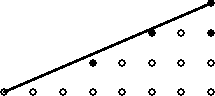
\includegraphics{pics/spin-377-pic-pics.pdf} \\
\caption{Generators in the $(\deg z, -ord_{P_i}(z))$ lattice}
\end{figure}

Also note that $e_j' + 2d = 7 + 2d \nmid 2 = e_i - e_j'$ for all
$i, j \in J_2 = \{2, 3\}$ such that $j \neq i$ and for all $d \geq
0$. Thus, $'s_{\sigma_2, J_2}(i, d) = \emptyset$ for each $i \in J$.
Furthermore, $\deg \lfloor e_i \halfcan \rfloor = \deg \lfloor 9
\halfcan \rfloor = 2 \lfloor \frac{4 * 9}{9} \rfloor + \lfloor
\frac{9}{3} \rfloor - 9 = 2$, so (Ad-iii) is satisfied and
$\sigma_2, J_2$ is admissible.
\end{example}

\begin{proof}
For the remaining cases, we can use a similar method to the one
used in Example ~\ref{ex:base-377} to find a presentation the
desired conditions.

The following table demonstrates that $R(\sx', \Delta, L')$ is
generated as a $k$-algebra by elements of degree at most $e$
with relations in degree at most $2e$ for each case. Also note
that in these cases, $e_i = e + 2 > \deg z$ for all $i \in J$
and any generator $z$ of $R'$.
\begin{longtable}
	{| c || c | c | c |}
	\hline
	Case & Generator Degrees & Degrees of Minimal Relations & $e$\\
	\hline
	\hline

	(a) & \{3, 7, 9, 11\} & \{14, 18\} & 11\\	\hline

	(b) & \{3, 5, 7, 9\} & \{12, 14\}	& 9\\ \hline

	(c) & \{3, 5, 7, 7\} & \{10, 14\}	& 7\\ \hline
	
	(d) & \{3, 5, 5, 7\} & \{10, 12\}	& 7\\ \hline
	
	(e) & \{3, 5, 5, 7, 7\} & \{10, 10, 12, 12, 14\}	& 7\\ \hline
	
	(f) & \{3, 5, 5, 7, 7, 7\} & \{10, 10, 10, 12, 12, 12, 14, 14, 14\}	& 7\\ \hline

	(g) & \{3, 3, 4, 5\} & \{8, 9\} & 5\\ \hline
	
	(h) & \{3, 3, 4, 5, 5\} & \{8, 8, 9, 9, 10\} & 5\\ \hline
	
	(i) & \{3, 3, 4, 5, 5, 5\} &
	\{8, 8, 8, 9, 9, 9, 10, 10, 10\} & 5\\ \hline
	
	(j) & \{3, 3, 4, 5, 5, 5, 5\} &
	\{8, 8, 8, 8, 9, 9, 9, 9, 10, 10, 10, 10, 10, 10\} & 5\\ \hline

	(k) &	\{3, 3, 3, 4,	4, 5\} & \{6, 7, 7, 8, 8, 8, 9, 9, 10\} & 5\\ \hline
\end{longtable}

\begin{center}
\textbf{Table (II)}: Genus 0 noneffective base cases generator/relations
\end{center}

We can also always find a presentation for these cases such that
they satisfy (Ad-i) and (Ad-ii) and that $in_\prec(I')$ is
minimally generated by products of two monomials. The procedure for
verifying these are similar to those for the given example.

Furthermore, each case always satisfies (Ad-iii) as demonstrated below.
Notice that the $e_i$ and $\{e_j' : j \neq i\}$ are equivalent
for any choice of $i \in J$ for these cases, so $\deg \lfloor e_i L
\rfloor$ and $\max_{d \geq 0} \#S_{(\sigma, J)}(i)$ are
independent of the choice of $i$.

\begin{longtable}
	{| c | c | c || c | c |}
	\hline
	Case & $\sigma$ & $J$ & $\deg \lfloor e_i L \rfloor$ &
	$\max_{d \geq 0} \#S_{(\sigma, J)}(i)$ \\
	\hline
	\hline

	(a) & $(0; 3, 3, 11; 0)$ & $\{3\}$ & 1 & 0 \\	\hline
	
	(b) & $(0; 3, 5, 9; 0)$ & $\{3\}$ & 1 & 0 \\ \hline
	
	(c) & $(0; 3, 7, 7; 0)$ & $\{3\}$ & 2 & 0 \\ \hline
	
	(d) & $(0; 5, 5, 7; 0)$ & $\{3\}$ & 1 & 0 \\ \hline
	
	(e) & $(0; 5, 7, 7; 0)$ & $\{2, 3\}$ & 2 & 0 \\ \hline

	(f) & $(0; 7, 7, 7; 0)$ & $\{1, 2, 3\}$ & 3 & 0 \\ \hline

	(g) & $(0; 3, 3, 3, 5; 0)$ & $\{4\}$ & 2 & 0 \\ \hline
	
	(h) & $(0; 3, 3, 5, 5; 0)$ & $\{3, 4\}$ & 3 & 0 \\ \hline
	
	(i) & $(0; 3, 5, 5, 5; 0)$ & $\{2, 3, 4\}$ & 4 & 0 \\ \hline
	
	(j) & $(0; 5, 5, 5, 5; 0)$ & $\{1, 2, 3, 4\}$ & 5 & 0 \\ \hline

	(k) & $(0; 3, 3, 3, 3, 3; 0)$ & $\{1, 2, 3, 4, 5\}$ & 5 & 0 \\ \hline
\end{longtable}

\begin{center}
\textbf{Table (III)}: Genus 0 noneffective base cases (Ad-iii)
\end{center}

Thus, all of the cases are admissible and satisfy the additional
desired conditions.
\end{proof}

Now we can induct on cases (a)-(k) of ~\ref{lem:g_0_admissible_cases}
to obtain bounds on the minimal generator and relation degrees for
canonical rings of curves in the genus 0 case.

Through the application of two processes of induction, by adding 
points via Lemma ~\ref{lem:sat-three-induction-g-0} and by raising
stabilizer orders via Theorem ~\ref{thm:ram_order_ind},
we obtain Theorem ~\ref{thm:g_0_generators_relations} for any
log spin curve $(\sx, \Delta, L)$ over a perfect field $k$ with
signature $\sigma$ covered by this induction process.
In particular, this induction process covers all signatures $\sigma
= (0; e_1, \ldots, e_r; 0)$ such that either $r \geq 5$ or
for some listed base case $(\sigma', J)$ with $\sigma' = (0; e_1',
\ldots, e_r'; 0)$, $e_i \geq e_i'$ for all $i$.
Before we prove the main theorem, we describe the cases not be
covered by induction.

\ssec{Exceptional Cases}
\label{ssec:g-0-exceptional}
First, we describe the cases that would not be covered by induction.
Here we present the explicit generators and relations of the remaining
cases given by signatures in the finite set

\begin{align*}
	S &:= \{(0; 3, 3, k; 0) : 3 \leq k \leq 9 \text{ odd}\} \\
		&\cup \{(0; 3, 5, 5; 0) ,(0; 3, 5, 7; 0), (0; 5, 5, 5; 0), (0; 3, 3, 3, 3; 0)\}
\end{align*}

\noindent
and in particular describe the only exceptions to the $e$ and $2e$
bounds on the generator degree and relation degree, respectively,
in the genus 0 case.

\begin{longtable}
	{| c || c | c | c |}
	\hline
	Signature & Generator Degrees & Degrees of Minimal Relations & $e$ \\
	\hline
	\hline

	$(0; 3, 3, 3; 0)$ & $\{3\}$ & $\emptyset$ & $3$ \\	\hline

	$(0; 3, 3, 5; 0)$ & $\{3, 10, 15\}$ & $\{30\}$ & $5$ \\	\hline
	
	$(0; 3, 3, 7; 0)$ & $\{3, 7, 12\}$ & $\{24\}$ & $7$ \\	\hline
	
	$(0; 3, 3, 9; 0)$ & $\{3, 7, 9\}$ & $\{21\}$ & $9$ \\	\hline
	
	$(0; 3, 5, 5; 0)$ & $\{3, 5, 10\}$ & $\{20\}$ & $5$ \\	\hline
	
	$(0; 3, 5, 7; 0)$ & $\{3, 5, 7\}$ & $\{17\}$ & $7$ \\	\hline
	
	$(0; 5, 5, 5; 0)$ & $\{3, 5, 5\}$ & $\{15\}$ & $5$ \\	\hline
	
	$(0; 3, 3, 3, 3; 0)$ & $\{3, 3, 4\}$ & $\{12\}$ & $3$ \\	\hline
\end{longtable}

\begin{center}
\label{table:g-0-exceptional}
\textbf{Table (IV)}: Genus 0 exceptional cases
\end{center}

\begin{rem}
These cases give all of the exceptions to the $e$ and $2e$ bounds on
the generator and relation degree. Notice that each of these
exceptional cases, apart from $(0; 3, 5, 7; 0)$, corresponds to a
signature with non-generic saturation (i.e. saturation not equal to
3, 5, or 9 as seen in the table in Subsection
~\ref{ssec:g_0_saturation}). Exceptional saturation can be viewed as
``forcing'' generators (and thus relations) in higher degrees than
in the generic case.
\end{rem}

\ssec{Main Theorem for Genus Zero}
\label{ssec:g_0_main}
Now we can combine this.
\todo{write this section}

\begin{thm}
\label{thm:g_0_generators_relations}
Let $(\sx, \Delta, \halfcan)$ log spin curve over a perfect field $k$,
so that $\sx$ has signature $\sigma = (0; e_1, \ldots, e_r; \delta)$.
If $g = 0$, then the canonical ring

\begin{align*}
	R(\sx, \Delta, \halfcan) = \bigoplus_{d = 0}^\infty H^0(\sx, \sco(L)^{\otimes d})
\end{align*}

\noindent
is generated as a $k$-algebra by elements of degree at most $e =
\max(5, e_1, \ldots, e_r)$ and has relations in degree at most $2e$,
so long as $\sigma$ does not lie in a finite list of exceptional
cases, as listed in Table ~\ref{table:g-0-exceptional}.
\end{thm}

\begin{proof}
If $\sx$ has no stacky points, then we can assume that $L \sim
n \cdot \infty$ with $n \in \BZ$. This is the classical
case which is done, with $L$ replaced by $K$, by Voight and
Zureick-Brown ~\cite[Section 4.2]{vzb:stacky}.

Now let us consider the case when $\delta \geq 2$. In any such case,
$\lfloor \halfcan \rfloor$ is an effective divisor and the conditions
of Lemma ~\ref{lem:deg1-sat-ind} are satisfied. Thus, we can apply
the lemma inductively on the classical case with no stacky points
to get that $R(\sx, \Delta, \halfcan)$ is generated up to degree $e$
with relations generated up to degree $2e$.

Now suppose $\delta = 0$, so $\halfcan$ is not necessarily effective.
Let $\sigma = (0; e_1, \ldots, e_r; 0)$ be a signature with $r > 0$
and not one of the exceptional cases in Table
~\ref{table:g-0-exceptional}.

If $r > 5$, then we can use Lemma
~\ref{lem:sat-three-induction-g-0} to add ramified points with
stabilizer order $3$ to case (k) of Lemma
~\ref{lem:g_0_admissible_cases}, which corresponds to $\sigma_{11}
= (0; 3, 3, 3, 3, 3; 0), J_{11} = \{1, 2, 3, 4, 5\}$. This case
clearly satisfies the conditions of Lemma
~\ref{lem:sat-three-induction-g-0} (recall from Subsection ~\ref
{ssec:g_0_saturation} that $\sat(\Eff(\sigma_{11})) = 3$), and the
immediate consequence of parts (a) and (c) of Lemma
~\ref{lem:sat-three-induction-g-0} is that any $R(\sx', \Delta,
\halfcan')$ corresponding to signatures $\sigma'$ with ramification
orders all equal to $3$ for any $r > 5$ is generated up to
degree $e := \max(5, e_1', \ldots, e_r')$ with relations generated
up to degree $2e$. Furthermore, these cases satisfy all of the
conditions of Theorem ~\ref{thm:ram_order_ind}.

So if $r > 5$, then $\sigma$ ``lies above'' the case $(\sigma', J)$
where $\sigma'$ has $r$ many stacky points all of order $3$
and $J = \{1, \ldots, r\}$ in the sense that for all $i
\in J$, $e_i \geq e_i'$ and $e_i = e_i'$ otherwise.
If $r \leq 5$, then $\sigma$ similarly ``lies above'' one of the
base cases of Lemma ~\ref{lem:g_0_admissible_cases}, all of which
satisfy the hypotheses of Theorem ~\ref{thm:ram_order_ind} as well.

So for any $r > 0$, there is a $(\sigma', J)$, either from
Lemma ~\ref{lem:g_0_admissible_cases} or corresponding to
the $r > 5$ case with stabilizer orders all $3$, with $\sigma' =
(0; e_1', \ldots, e_r'; 0)$ satisfying the property that for all $i
\in J$, $e_i \geq e_i'$ and $e_i = e_i'$ otherwise.

All such base cases satisfy all of the hypotheses of
Theorem ~\ref{thm:ram_order_ind} and their corresponding $R' :=
R(\sx', \Delta, \halfcan')$ are generated, as $k$-algebras, up
to degree $e' := \max(5, e_1', \ldots, e_r')$ with relations
generated up to degree $2e'$ by Lemma ~\ref{lem:g_0_admissible_cases}.
It follows from Theorem ~\ref{thm:ram_order_ind}(b) that $R :=
R(\sx, \Delta, \halfcan)$ is generated up to degree $e := \max(5,
e_1, \ldots, e_r)$. It follows from Theorem ~\ref{thm:ram_order_ind}
(d) that the relations are generated up to degree $2e$.
\end{proof}

\section{Further Research}
\label{sec:further-questions}
\begin{itemize}
	\item More on fractional modular forms
	\item Make explicit generators and relations for base case of non-stacky higher genus half-canonical divisors
	\item In the case $g \geq 2$, can the bound from Proposition ~\ref{prop:relation_11} be reduced from 11 to 10 (which would then be sharp by Remark ~\ref{rem:relations_generation_ten})? \todo{Possibly think more about this} 
	\item Generic Initial ideal (and other genericness properties?)
	\item Complete minimal generation
\end{itemize}

%%%%%%%%%%%%%%%%%%%%%%%%% Acknowledgements %%%%%%%%%%%%%%%%%%%%%%%%%%%%

\section{Acknowledgments}
We are grateful to David Zureick-Brown for introducing us to this
field of study, providing incredibly helpful guidance, and being an
excellent project mentor. We also thank Ken Ono and the Emory University
Number Theory REU for arranging our project and providing a great
environment for mathematical learning and collaboration. Finally, we
gratefully acknowledge that our research was financially supported by
NSF Grant Award Number 1250467 via the Emory University Number Theory REU.
We deeply appreciate all of the support that has made our work possible.

%%%%%%%%%%%%%%%%%%%%%%%%%%%% References %%%%%%%%%%%%%%%%%%%%%%%%%%%%%%%

\nocite{*}
\bibliography{bibliography}{}
\bibliographystyle{plain}

\end{document}